% Sample LaTeX file for creating a paper in the Morgan Kaufmannn two
% column, 8 1/2 by 11 inch proceedings format.

\documentclass[letterpaper]{article}
\usepackage{uai2019}
\usepackage[margin=1in]{geometry}

% Set the typeface to Times Roman
\usepackage{times}

% Optional math commands from https://github.com/goodfeli/dlbook_notation.
%%%%% NEW MATH DEFINITIONS %%%%%

\usepackage{amsmath,amsfonts,bm}

% Mark sections of captions for referring to divisions of figures
\newcommand{\figleft}{{\em (Left)}}
\newcommand{\figcenter}{{\em (Center)}}
\newcommand{\figright}{{\em (Right)}}
\newcommand{\figtop}{{\em (Top)}}
\newcommand{\figbottom}{{\em (Bottom)}}
\newcommand{\captiona}{{\em (a)}}
\newcommand{\captionb}{{\em (b)}}
\newcommand{\captionc}{{\em (c)}}
\newcommand{\captiond}{{\em (d)}}

% Highlight a newly defined term
\newcommand{\newterm}[1]{{\bf #1}}


% Figure reference, lower-case.
\def\figref#1{figure~\ref{#1}}
% Figure reference, capital. For start of sentence
\def\Figref#1{Figure~\ref{#1}}
\def\twofigref#1#2{figures \ref{#1} and \ref{#2}}
\def\quadfigref#1#2#3#4{figures \ref{#1}, \ref{#2}, \ref{#3} and \ref{#4}}
% Section reference, lower-case.
\def\secref#1{section~\ref{#1}}
% Section reference, capital.
\def\Secref#1{Section~\ref{#1}}
% Reference to two sections.
\def\twosecrefs#1#2{sections \ref{#1} and \ref{#2}}
% Reference to three sections.
\def\secrefs#1#2#3{sections \ref{#1}, \ref{#2} and \ref{#3}}
% Reference to an equation, lower-case.
\def\eqref#1{equation~\ref{#1}}
% Reference to an equation, upper case
\def\Eqref#1{Equation~\ref{#1}}
% A raw reference to an equation---avoid using if possible
\def\plaineqref#1{\ref{#1}}
% Reference to a chapter, lower-case.
\def\chapref#1{chapter~\ref{#1}}
% Reference to an equation, upper case.
\def\Chapref#1{Chapter~\ref{#1}}
% Reference to a range of chapters
\def\rangechapref#1#2{chapters\ref{#1}--\ref{#2}}
% Reference to an algorithm, lower-case.
\def\algref#1{algorithm~\ref{#1}}
% Reference to an algorithm, upper case.
\def\Algref#1{Algorithm~\ref{#1}}
\def\twoalgref#1#2{algorithms \ref{#1} and \ref{#2}}
\def\Twoalgref#1#2{Algorithms \ref{#1} and \ref{#2}}
% Reference to a part, lower case
\def\partref#1{part~\ref{#1}}
% Reference to a part, upper case
\def\Partref#1{Part~\ref{#1}}
\def\twopartref#1#2{parts \ref{#1} and \ref{#2}}

\def\ceil#1{\lceil #1 \rceil}
\def\floor#1{\lfloor #1 \rfloor}
\def\1{\bm{1}}
\newcommand{\train}{\mathcal{D}}
\newcommand{\valid}{\mathcal{D_{\mathrm{valid}}}}
\newcommand{\test}{\mathcal{D_{\mathrm{test}}}}

\def\eps{{\epsilon}}


% Random variables
\def\reta{{\textnormal{$\eta$}}}
\def\ra{{\textnormal{a}}}
\def\rb{{\textnormal{b}}}
\def\rc{{\textnormal{c}}}
\def\rd{{\textnormal{d}}}
\def\re{{\textnormal{e}}}
\def\rf{{\textnormal{f}}}
\def\rg{{\textnormal{g}}}
\def\rh{{\textnormal{h}}}
\def\ri{{\textnormal{i}}}
\def\rj{{\textnormal{j}}}
\def\rk{{\textnormal{k}}}
\def\rl{{\textnormal{l}}}
% rm is already a command, just don't name any random variables m
\def\rn{{\textnormal{n}}}
\def\ro{{\textnormal{o}}}
\def\rp{{\textnormal{p}}}
\def\rq{{\textnormal{q}}}
\def\rr{{\textnormal{r}}}
\def\rs{{\textnormal{s}}}
\def\rt{{\textnormal{t}}}
\def\ru{{\textnormal{u}}}
\def\rv{{\textnormal{v}}}
\def\rw{{\textnormal{w}}}
\def\rx{{\textnormal{x}}}
\def\ry{{\textnormal{y}}}
\def\rz{{\textnormal{z}}}

% Random vectors
\def\rvepsilon{{\mathbf{\epsilon}}}
\def\rvtheta{{\mathbf{\theta}}}
\def\rva{{\mathbf{a}}}
\def\rvb{{\mathbf{b}}}
\def\rvc{{\mathbf{c}}}
\def\rvd{{\mathbf{d}}}
\def\rve{{\mathbf{e}}}
\def\rvf{{\mathbf{f}}}
\def\rvg{{\mathbf{g}}}
\def\rvh{{\mathbf{h}}}
\def\rvu{{\mathbf{i}}}
\def\rvj{{\mathbf{j}}}
\def\rvk{{\mathbf{k}}}
\def\rvl{{\mathbf{l}}}
\def\rvm{{\mathbf{m}}}
\def\rvn{{\mathbf{n}}}
\def\rvo{{\mathbf{o}}}
\def\rvp{{\mathbf{p}}}
\def\rvq{{\mathbf{q}}}
\def\rvr{{\mathbf{r}}}
\def\rvs{{\mathbf{s}}}
\def\rvt{{\mathbf{t}}}
\def\rvu{{\mathbf{u}}}
\def\rvv{{\mathbf{v}}}
\def\rvw{{\mathbf{w}}}
\def\rvx{{\mathbf{x}}}
\def\rvy{{\mathbf{y}}}
\def\rvz{{\mathbf{z}}}

% Elements of random vectors
\def\erva{{\textnormal{a}}}
\def\ervb{{\textnormal{b}}}
\def\ervc{{\textnormal{c}}}
\def\ervd{{\textnormal{d}}}
\def\erve{{\textnormal{e}}}
\def\ervf{{\textnormal{f}}}
\def\ervg{{\textnormal{g}}}
\def\ervh{{\textnormal{h}}}
\def\ervi{{\textnormal{i}}}
\def\ervj{{\textnormal{j}}}
\def\ervk{{\textnormal{k}}}
\def\ervl{{\textnormal{l}}}
\def\ervm{{\textnormal{m}}}
\def\ervn{{\textnormal{n}}}
\def\ervo{{\textnormal{o}}}
\def\ervp{{\textnormal{p}}}
\def\ervq{{\textnormal{q}}}
\def\ervr{{\textnormal{r}}}
\def\ervs{{\textnormal{s}}}
\def\ervt{{\textnormal{t}}}
\def\ervu{{\textnormal{u}}}
\def\ervv{{\textnormal{v}}}
\def\ervw{{\textnormal{w}}}
\def\ervx{{\textnormal{x}}}
\def\ervy{{\textnormal{y}}}
\def\ervz{{\textnormal{z}}}

% Random matrices
\def\rmA{{\mathbf{A}}}
\def\rmB{{\mathbf{B}}}
\def\rmC{{\mathbf{C}}}
\def\rmD{{\mathbf{D}}}
\def\rmE{{\mathbf{E}}}
\def\rmF{{\mathbf{F}}}
\def\rmG{{\mathbf{G}}}
\def\rmH{{\mathbf{H}}}
\def\rmI{{\mathbf{I}}}
\def\rmJ{{\mathbf{J}}}
\def\rmK{{\mathbf{K}}}
\def\rmL{{\mathbf{L}}}
\def\rmM{{\mathbf{M}}}
\def\rmN{{\mathbf{N}}}
\def\rmO{{\mathbf{O}}}
\def\rmP{{\mathbf{P}}}
\def\rmQ{{\mathbf{Q}}}
\def\rmR{{\mathbf{R}}}
\def\rmS{{\mathbf{S}}}
\def\rmT{{\mathbf{T}}}
\def\rmU{{\mathbf{U}}}
\def\rmV{{\mathbf{V}}}
\def\rmW{{\mathbf{W}}}
\def\rmX{{\mathbf{X}}}
\def\rmY{{\mathbf{Y}}}
\def\rmZ{{\mathbf{Z}}}

% Elements of random matrices
\def\ermA{{\textnormal{A}}}
\def\ermB{{\textnormal{B}}}
\def\ermC{{\textnormal{C}}}
\def\ermD{{\textnormal{D}}}
\def\ermE{{\textnormal{E}}}
\def\ermF{{\textnormal{F}}}
\def\ermG{{\textnormal{G}}}
\def\ermH{{\textnormal{H}}}
\def\ermI{{\textnormal{I}}}
\def\ermJ{{\textnormal{J}}}
\def\ermK{{\textnormal{K}}}
\def\ermL{{\textnormal{L}}}
\def\ermM{{\textnormal{M}}}
\def\ermN{{\textnormal{N}}}
\def\ermO{{\textnormal{O}}}
\def\ermP{{\textnormal{P}}}
\def\ermQ{{\textnormal{Q}}}
\def\ermR{{\textnormal{R}}}
\def\ermS{{\textnormal{S}}}
\def\ermT{{\textnormal{T}}}
\def\ermU{{\textnormal{U}}}
\def\ermV{{\textnormal{V}}}
\def\ermW{{\textnormal{W}}}
\def\ermX{{\textnormal{X}}}
\def\ermY{{\textnormal{Y}}}
\def\ermZ{{\textnormal{Z}}}

% Vectors
\def\vzero{{\bm{0}}}
\def\vone{{\bm{1}}}
\def\vmu{{\bm{\mu}}}
\def\vtheta{{\bm{\theta}}}
\def\va{{\bm{a}}}
\def\vb{{\bm{b}}}
\def\vc{{\bm{c}}}
\def\vd{{\bm{d}}}
\def\ve{{\bm{e}}}
\def\vf{{\bm{f}}}
\def\vg{{\bm{g}}}
\def\vh{{\bm{h}}}
\def\vi{{\bm{i}}}
\def\vj{{\bm{j}}}
\def\vk{{\bm{k}}}
\def\vl{{\bm{l}}}
\def\vm{{\bm{m}}}
\def\vn{{\bm{n}}}
\def\vo{{\bm{o}}}
\def\vp{{\bm{p}}}
\def\vq{{\bm{q}}}
\def\vr{{\bm{r}}}
\def\vs{{\bm{s}}}
\def\vt{{\bm{t}}}
\def\vu{{\bm{u}}}
\def\vv{{\bm{v}}}
\def\vw{{\bm{w}}}
\def\vx{{\bm{x}}}
\def\vy{{\bm{y}}}
\def\vz{{\bm{z}}}

% Elements of vectors
\def\evalpha{{\alpha}}
\def\evbeta{{\beta}}
\def\evepsilon{{\epsilon}}
\def\evlambda{{\lambda}}
\def\evomega{{\omega}}
\def\evmu{{\mu}}
\def\evpsi{{\psi}}
\def\evsigma{{\sigma}}
\def\evtheta{{\theta}}
\def\eva{{a}}
\def\evb{{b}}
\def\evc{{c}}
\def\evd{{d}}
\def\eve{{e}}
\def\evf{{f}}
\def\evg{{g}}
\def\evh{{h}}
\def\evi{{i}}
\def\evj{{j}}
\def\evk{{k}}
\def\evl{{l}}
\def\evm{{m}}
\def\evn{{n}}
\def\evo{{o}}
\def\evp{{p}}
\def\evq{{q}}
\def\evr{{r}}
\def\evs{{s}}
\def\evt{{t}}
\def\evu{{u}}
\def\evv{{v}}
\def\evw{{w}}
\def\evx{{x}}
\def\evy{{y}}
\def\evz{{z}}

% Matrix
\def\mA{{\bm{A}}}
\def\mB{{\bm{B}}}
\def\mC{{\bm{C}}}
\def\mD{{\bm{D}}}
\def\mE{{\bm{E}}}
\def\mF{{\bm{F}}}
\def\mG{{\bm{G}}}
\def\mH{{\bm{H}}}
\def\mI{{\bm{I}}}
\def\mJ{{\bm{J}}}
\def\mK{{\bm{K}}}
\def\mL{{\bm{L}}}
\def\mM{{\bm{M}}}
\def\mN{{\bm{N}}}
\def\mO{{\bm{O}}}
\def\mP{{\bm{P}}}
\def\mQ{{\bm{Q}}}
\def\mR{{\bm{R}}}
\def\mS{{\bm{S}}}
\def\mT{{\bm{T}}}
\def\mU{{\bm{U}}}
\def\mV{{\bm{V}}}
\def\mW{{\bm{W}}}
\def\mX{{\bm{X}}}
\def\mY{{\bm{Y}}}
\def\mZ{{\bm{Z}}}
\def\mBeta{{\bm{\beta}}}
\def\mPhi{{\bm{\Phi}}}
\def\mLambda{{\bm{\Lambda}}}
\def\mSigma{{\bm{\Sigma}}}

% Tensor
\DeclareMathAlphabet{\mathsfit}{\encodingdefault}{\sfdefault}{m}{sl}
\SetMathAlphabet{\mathsfit}{bold}{\encodingdefault}{\sfdefault}{bx}{n}
\newcommand{\tens}[1]{\bm{\mathsfit{#1}}}
\def\tA{{\tens{A}}}
\def\tB{{\tens{B}}}
\def\tC{{\tens{C}}}
\def\tD{{\tens{D}}}
\def\tE{{\tens{E}}}
\def\tF{{\tens{F}}}
\def\tG{{\tens{G}}}
\def\tH{{\tens{H}}}
\def\tI{{\tens{I}}}
\def\tJ{{\tens{J}}}
\def\tK{{\tens{K}}}
\def\tL{{\tens{L}}}
\def\tM{{\tens{M}}}
\def\tN{{\tens{N}}}
\def\tO{{\tens{O}}}
\def\tP{{\tens{P}}}
\def\tQ{{\tens{Q}}}
\def\tR{{\tens{R}}}
\def\tS{{\tens{S}}}
\def\tT{{\tens{T}}}
\def\tU{{\tens{U}}}
\def\tV{{\tens{V}}}
\def\tW{{\tens{W}}}
\def\tX{{\tens{X}}}
\def\tY{{\tens{Y}}}
\def\tZ{{\tens{Z}}}


% Graph
\def\gA{{\mathcal{A}}}
\def\gB{{\mathcal{B}}}
\def\gC{{\mathcal{C}}}
\def\gD{{\mathcal{D}}}
\def\gE{{\mathcal{E}}}
\def\gF{{\mathcal{F}}}
\def\gG{{\mathcal{G}}}
\def\gH{{\mathcal{H}}}
\def\gI{{\mathcal{I}}}
\def\gJ{{\mathcal{J}}}
\def\gK{{\mathcal{K}}}
\def\gL{{\mathcal{L}}}
\def\gM{{\mathcal{M}}}
\def\gN{{\mathcal{N}}}
\def\gO{{\mathcal{O}}}
\def\gP{{\mathcal{P}}}
\def\gQ{{\mathcal{Q}}}
\def\gR{{\mathcal{R}}}
\def\gS{{\mathcal{S}}}
\def\gT{{\mathcal{T}}}
\def\gU{{\mathcal{U}}}
\def\gV{{\mathcal{V}}}
\def\gW{{\mathcal{W}}}
\def\gX{{\mathcal{X}}}
\def\gY{{\mathcal{Y}}}
\def\gZ{{\mathcal{Z}}}

% Sets
\def\sA{{\mathbb{A}}}
\def\sB{{\mathbb{B}}}
\def\sC{{\mathbb{C}}}
\def\sD{{\mathbb{D}}}
% Don't use a set called E, because this would be the same as our symbol
% for expectation.
\def\sF{{\mathbb{F}}}
\def\sG{{\mathbb{G}}}
\def\sH{{\mathbb{H}}}
\def\sI{{\mathbb{I}}}
\def\sJ{{\mathbb{J}}}
\def\sK{{\mathbb{K}}}
\def\sL{{\mathbb{L}}}
\def\sM{{\mathbb{M}}}
\def\sN{{\mathbb{N}}}
\def\sO{{\mathbb{O}}}
\def\sP{{\mathbb{P}}}
\def\sQ{{\mathbb{Q}}}
\def\sR{{\mathbb{R}}}
\def\sS{{\mathbb{S}}}
\def\sT{{\mathbb{T}}}
\def\sU{{\mathbb{U}}}
\def\sV{{\mathbb{V}}}
\def\sW{{\mathbb{W}}}
\def\sX{{\mathbb{X}}}
\def\sY{{\mathbb{Y}}}
\def\sZ{{\mathbb{Z}}}

% Entries of a matrix
\def\emLambda{{\Lambda}}
\def\emA{{A}}
\def\emB{{B}}
\def\emC{{C}}
\def\emD{{D}}
\def\emE{{E}}
\def\emF{{F}}
\def\emG{{G}}
\def\emH{{H}}
\def\emI{{I}}
\def\emJ{{J}}
\def\emK{{K}}
\def\emL{{L}}
\def\emM{{M}}
\def\emN{{N}}
\def\emO{{O}}
\def\emP{{P}}
\def\emQ{{Q}}
\def\emR{{R}}
\def\emS{{S}}
\def\emT{{T}}
\def\emU{{U}}
\def\emV{{V}}
\def\emW{{W}}
\def\emX{{X}}
\def\emY{{Y}}
\def\emZ{{Z}}
\def\emSigma{{\Sigma}}

% entries of a tensor
% Same font as tensor, without \bm wrapper
\newcommand{\etens}[1]{\mathsfit{#1}}
\def\etLambda{{\etens{\Lambda}}}
\def\etA{{\etens{A}}}
\def\etB{{\etens{B}}}
\def\etC{{\etens{C}}}
\def\etD{{\etens{D}}}
\def\etE{{\etens{E}}}
\def\etF{{\etens{F}}}
\def\etG{{\etens{G}}}
\def\etH{{\etens{H}}}
\def\etI{{\etens{I}}}
\def\etJ{{\etens{J}}}
\def\etK{{\etens{K}}}
\def\etL{{\etens{L}}}
\def\etM{{\etens{M}}}
\def\etN{{\etens{N}}}
\def\etO{{\etens{O}}}
\def\etP{{\etens{P}}}
\def\etQ{{\etens{Q}}}
\def\etR{{\etens{R}}}
\def\etS{{\etens{S}}}
\def\etT{{\etens{T}}}
\def\etU{{\etens{U}}}
\def\etV{{\etens{V}}}
\def\etW{{\etens{W}}}
\def\etX{{\etens{X}}}
\def\etY{{\etens{Y}}}
\def\etZ{{\etens{Z}}}

% The true underlying data generating distribution
\newcommand{\pdata}{p_{\rm{data}}}
% The empirical distribution defined by the training set
\newcommand{\ptrain}{\hat{p}_{\rm{data}}}
\newcommand{\Ptrain}{\hat{P}_{\rm{data}}}
% The model distribution
\newcommand{\pmodel}{p_{\rm{model}}}
\newcommand{\Pmodel}{P_{\rm{model}}}
\newcommand{\ptildemodel}{\tilde{p}_{\rm{model}}}
% Stochastic autoencoder distributions
\newcommand{\pencode}{p_{\rm{encoder}}}
\newcommand{\pdecode}{p_{\rm{decoder}}}
\newcommand{\precons}{p_{\rm{reconstruct}}}

\newcommand{\laplace}{\mathrm{Laplace}} % Laplace distribution

\newcommand{\E}{\mathbb{E}}
\newcommand{\Ls}{\mathcal{L}}
\newcommand{\R}{\mathbb{R}}
\newcommand{\emp}{\tilde{p}}
\newcommand{\lr}{\alpha}
\newcommand{\reg}{\lambda}
\newcommand{\rect}{\mathrm{rectifier}}
\newcommand{\softmax}{\mathrm{softmax}}
\newcommand{\sigmoid}{\sigma}
\newcommand{\softplus}{\zeta}
\newcommand{\KL}{D_{\mathrm{KL}}}
\newcommand{\Var}{\mathrm{Var}}
\newcommand{\standarderror}{\mathrm{SE}}
\newcommand{\Cov}{\mathrm{Cov}}
% Wolfram Mathworld says $L^2$ is for function spaces and $\ell^2$ is for vectors
% But then they seem to use $L^2$ for vectors throughout the site, and so does
% wikipedia.
\newcommand{\normlzero}{L^0}
\newcommand{\normlone}{L^1}
\newcommand{\normltwo}{L^2}
\newcommand{\normlp}{L^p}
\newcommand{\normmax}{L^\infty}

\newcommand{\parents}{Pa} % See usage in notation.tex. Chosen to match Daphne's book.

\DeclareMathOperator*{\argmax}{arg\,max}
\DeclareMathOperator*{\argmin}{arg\,min}

\DeclareMathOperator{\sign}{sign}
\DeclareMathOperator{\Tr}{Tr}
\let\ab\allowbreak


\usepackage[numbers,sort&compress]{natbib}
\usepackage{hyperref}
\usepackage{url}
\usepackage{paralist}
\usepackage[acronym,smallcaps,nowarn,section,nogroupskip,nonumberlist]{glossaries}
\usepackage[nameinlink,capitalise]{cleveref}
\usepackage{amssymb}
\usepackage{mathtools}
\usepackage{tikz}
\usepackage{etoolbox}
\usepackage{graphicx}
\usepackage{wrapfig}
\usepackage[font=small]{caption}
\usepackage{subcaption}
\usepackage{booktabs}
\usepackage{titlesec}
\usepackage[textsize=footnotesize]{todonotes}
\usepackage{balance}
\usepackage[ruled,vlined]{algorithm2e}

%% Colours
\definecolor{red}{HTML}{E41A1C}
\definecolor{orange}{HTML}{FF7F00}
\definecolor{yellow}{HTML}{FFC020}
\definecolor{green}{HTML}{4DAF4A}
\definecolor{blue}{HTML}{377EB8}
\definecolor{purple}{HTML}{984EA3}
% tikz
\usetikzlibrary{calc,backgrounds,positioning,bayesnet,arrows.meta,patterns,fit,trees}
% todo
\presetkeys{todonotes}{%
  backgroundcolor=blue!10!white,
  linecolor=blue!10!white,
  bordercolor=blue!10!white
}{}
% cleveref
\Crefname{algocf}{Algorithm}{Algorithms}
\crefname{algorithm}{Algorithm}{Algorithms}
% \crefname{equation}{Equation}{Equations}
\crefname{figure}{Figure}{Figure}
\crefname{table}{Table}{Table}
\crefname{section}{\S}{\S\S}
\Crefname{section}{\S}{\S\S}
\crefformat{equation}{(#2#1#3)}
% abbreviations
% must run `makeglossaries main'
% https://tex.stackexchange.com/questions/43759/printglossaries-is-not-generating-anything-for-me
\makeglossaries
\glsdisablehyper{}
\newacronym{SCFM}{scfm}{stochastic control-flow model}
\newacronym{WS}{ws}{wake-sleep}
\newacronym{BWS}{bws}{basic wake-sleep}
\newacronym{RWS}{rws}{reweighted wake-sleep}
\newacronym{ELBO}{elbo}{evidence lower bound}
\newacronym{VAE}{vae}{variational autoencoder}
\newacronym{IWAE}{iwae}{importance weighted autoencoder}
\newacronym{KL}{kl}{Kullback-Leibler}
\newacronym{SGD}{sgd}{stochastic gradient descent}
\newacronym{VIMCO}{vimco}{variational inference for Monte Carlo objectives}
\newacronym{WW}{ww}{wake-wake}
\newacronym{WWS}{wws}{wake-wake-sleep}
\newacronym{AIR}{air}{Attend, Infer, Repeat}
\newacronym{ESS}{ess}{effective sample size}
\newacronym{REINFORCE}{reinforce}{Reinforce gradient estimator}
\newacronym{IS}{is}{importance sampling}
\newacronym{GMM}{gmm}{Gaussian mixture model}
\newacronym{MNIST}{mnist}{hand-written digit dataset}
\newacronym{RELAX}{relax}{RELAX gradient estimator}
\newacronym{REBAR}{rebar}{REBAR gradient estimator}
\newacronym{PMF}{pmf}{probability mass function}
\newacronym{MLP}{mlp}{multilayer perceptron}
\newacronym{RNN}{rnn}{recurrent neural network}
\newacronym{PCFG}{pcfg}{probabilistic context free grammar}
\newacronym{ADAM}{adam}{ADAM}
\glsunset{ADAM}
% titlesec
% \titlespacing\section{0pt}{3pt plus 4pt minus 2pt}{0pt plus 2pt minus 2pt}
% \titlespacing\subsection{0pt}{3pt plus 4pt minus 2pt}{0pt plus 2pt minus 2pt}

\makeatletter
\renewcommand\paragraph{\@startsection{paragraph}{4}{\z@}%
 {0ex \@plus1ex \@minus.2ex}%
 {-1em}%
 {\normalfont\normalsize\bfseries}}
\makeatother

\newcommand{\circled}[2][]{%
  \tikz[baseline=(char.base)]{%
    \node[shape = circle, draw, inner sep = 1pt,scale=0.75]
    (char) {\phantom{\ifblank{#1}{#2}{#1}}};%
    \node at (char.center) {\makebox[0pt][c]{\scriptsize #2}};}}
\robustify{\circled}

% math
\newcommand{\given}{\lvert}
\DeclareMathOperator{\ELBO}{\acrshort{ELBO}}
\DeclareMathOperator{\std}{\mathrm{std}}

\newcommand{\ak}[1]{\textcolor{blue}{\textbf{ak}: #1}}
\newcommand{\sid}[1]{\todo{sid:#1}}
\newcommand{\tal}[1]{\todo{tal:#1}}

\hyphenation{app-roach}
\hyphenation{auto-encoder}

\title{Revisiting Reweighted Wake-Sleep \\[0.5ex]
for Models with Stochastic Control Flow}

% \author{} % LEAVE BLANK FOR ORIGINAL SUBMISSION.
%           % UAI  reviewing is double-blind.

% The author names and affiliations should appear only in the accepted paper.
%
\author{
  Tuan~Anh Le$^1$\thanks{\quad Equal contribution.} \quad Adam R. Kosiorek$^{1, 2}$\footnotemark[1] \quad N. Siddharth$^1$\quad Yee~Whye Teh$^2$\quad Frank Wood$^3$\\
  $^1$ Department of Engineering Science, University of Oxford \\
  $^2$ Department of Statistics, University of Oxford \\
  $^3$ Department of Computer Science, University of British Columbia
  % \texttt{\{tuananh,adamk,nsid\}@robots.ox.ac.uk,y.w.teh@stats.ox.ac.uk,fwood@cs.ubc.ca}
}

\begin{document}

\maketitle

\begin{abstract}
  \Glspl{SCFM} are a class of generative models that involve branching on choices from discrete random variables.
  %
  Amortized gradient-based learning of \glspl{SCFM} is challenging as most approaches targeting discrete variables rely on their continuous relaxations---which can be intractable in \glspl{SCFM}, as branching on relaxations requires evaluating \emph{all} (exponentially many) branching paths.
  %
  Tractable alternatives mainly combine \acrshort{REINFORCE} with complex control-variate schemes to improve the variance of na\"ive estimators.
  %
  Here, we revisit the \gls{RWS}~\citep{bornschein2015reweighted} algorithm, and through extensive evaluations, show that it outperforms current state-of-the-art methods in learning \glspl{SCFM}.
  %
  Further, in contrast to the \acrlong{IWAE}, we observe that \gls{RWS} learns better models \emph{and} inference networks with increasing numbers of particles.
  %
  Our results suggest that \gls{RWS} is a competitive, often preferable, alternative for learning \glspl{SCFM}.
\end{abstract}

\glsresetall
% !tex root=./main.tex
\vspace*{-1\baselineskip}
\section{INTRODUCTION}
\label{sec:introduction}

\Glspl{SCFM} describe generative models that employ branching (i.e., the use of {\small \texttt{if} / \texttt{else} / \texttt{cond}} statements) on choices from discrete random variables.
%
Recent years have seen such models gain relevance, particularly in the domain of deep probabilistic programming~\citep[Ch. 7]{siddharth2017learning,bingham2019pyro,tran2017deep,vandemeent2018intro}, which allows combining neural networks with generative models expressing arbitrarily complex control flow.
%
\Glspl{SCFM} are encountered in a wide variety of tasks including tracking and prediction \citep{neiswanger2014dependent,kosiorek2018sequential}, clustering \citep{rasmussen2000infinite}, topic modeling \citep{blei2003latent}, model structure learning \citep{adams2010learning}, counting \citep{eslami2016attend}, attention \citep{xu2015show}, differentiable data structures \citep{graves2014neural,graves2016hybrid,grefenstette2015learning}, speech \& language modeling \citep{juang1991hidden,chater2006probabilistic}, and concept learning \citep{kemp2006learning,lake2018emergence}.

While a variety of approaches for amortized gradient-based learning (targeting model \gls{ELBO}) exist for models using discrete random variables, the majority rely on continuous relaxations of the discrete variables~\citep[e.g.][]{rolfe2016dvae,vahdat2018dvaepp,vahdat2018dvaehash,oord2017neural,maddison2017concrete,jang2017categorical}, enabling gradient computation through reparameterization~\citep{kingma2014auto,rezende2014stochastic}.
%
The models used by these approaches typically do not involve any control flow on discrete random choices, instead choosing to feed choices from their continuous relaxations directly into a neural network, thereby facilitating the required learning.


\begin{figure}[t]
  \centering
  \scriptsize
  \def\figuresize{5mm}
  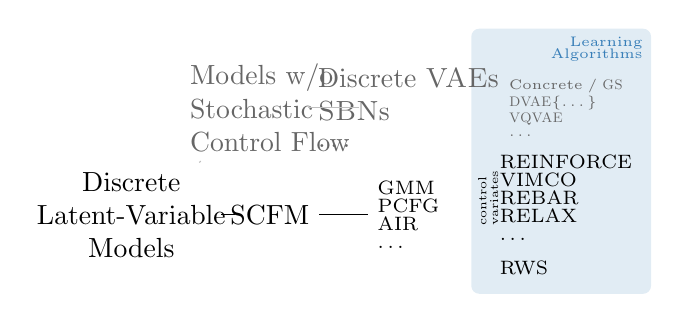
\begin{tikzpicture}[%
    scale=0.8,
    txt/.style={text centered},
    infs/.style={txt,align=left,font=\tiny},
    bgb/.style={rounded corners=1mm,minimum height=1.5cm,minimum width=2cm},
    level 1/.style={sibling distance=1.7cm, level distance=2.2cm},
    level 2/.style={sibling distance=1cm, level distance=2.2cm},
    level 3/.style={level distance=2.5cm},
    grow=right,
    ]
    \node[txt,align=center] {Discrete\\Latent-Variable\\Models}
    child[missing]              % dummy child for spacing
    child {                     % SCFMs
      node[txt] {\acrshortpl{SCFM}}
      child {
        node[txt,align=left,font=\scriptsize] (eg2) {
          \acrshort{GMM}\\[-0.5ex]
          \acrshort{PCFG}\\[-0.5ex]
          \acrshort{AIR}\\[-0.5ex]
          \ldots
        }
        child {
          node[infs,font=\scriptsize] (cvs) {
            \acrshort{REINFORCE}\\[-0.5ex]
            \acrshort{VIMCO}\\[-0.5ex]
            \acrshort{REBAR}\\[-0.5ex]
            \acrshort{RELAX}\\[-0.5ex]
            \ldots\\[1.5ex]
            \acrshort{RWS}
          }
          edge from parent[draw=none]
          node[above,font=\tiny,scale=0.85,align=left,
               rotate=90,xshift=2.5mm,yshift=-5.5mm]{control\\[-0.5ex]variates}
        }
      }
    }
    child {                     % non-SCFMs
      node[txt,align=left,text=gray!80!black] {Models w/o\\Stochastic\\Control Flow}
      child {
        node[txt,text=gray!80!black,align=left] (eg1) {
          Discrete \textsc{VAE}s\\
          \textsc{SBN}s\\[-0.5ex]
          \ldots
        }
        child {
          node[infs,text=gray!80!black] (others) {
            Concrete\;/\;\textsc{GS}\\
            \textsc{DVAE}\{\ldots\}\\
            \textsc{VQVAE}\\[-0.5ex]
            \ldots
          }
         edge from parent[draw=none]
        }
      }
      edge from parent[draw=gray!50]
    };
    \scoped[on background layer]
    \node[bgb, fill=blue!15, fit={($(others.north west)+(-3mm,5mm)$)($(cvs.south east)$)},
    label={[xshift=4.5mm,yshift=-5.5mm,align=right,font=\tiny,text=blue]above:
            Learning\\[-0.5mm]Algorithms}
    ] {};
  \end{tikzpicture}
  \vspace*{-0.5\baselineskip}
  \caption{An overview of learning algorithms for discrete latent-variable models, with focus on \glspl{SCFM}.}
  \label{fig:scfm}
  \vspace*{-2.7\baselineskip}
\end{figure}

In contrast, \glspl{SCFM} do not lend themselves to continuous-relaxation-based approaches due to the explicit branching requirement on choices from the discrete variables.
%
Consider for example a simple \gls{SCFM}---a two-mixture \gls{GMM}.
%
Computing the \gls{ELBO} for this model involves choosing mixture identity (Bernoulli).
%
Since a sample from a relaxed variable denotes a point on the surface of a probability simplex (e.g. [0.2, 0.8] for a Bernoulli random variable), instead of its vertices (0 or 1), computing the \gls{ELBO} would need evaluation of both branches, weighting the resulting computation under each branch appropriately.
%
This process can very quickly become intractable for more complex \glspl{SCFM}, as it requires evaluation of \emph{all} possible branches in the computation, of which there may be \emph{exponentially} many, as illustrated in \cref{fig:exponential-all}.
%
% sid: include the biased gradient estimator angle here?

Alternatives to continuous-relaxation methods mainly involve the use of the \gls{IWAE}~\citep{burda2016importance} framework, employing the \acrshort{REINFORCE}~\citep{williams1992simple} gradient estimator, combined with control-variate schemes~\citep{mnih2014neural,mnih2016variational,gu2016muprop,tucker2017rebar,grathwohl2018backpropagation} to help decrease the variance of the na\"ive estimator.
%
Although this approach ameliorates the problem with continuous relaxations in that it does not require evaluation of all branches, it has other drawbacks.
%
Firstly, with more particles, the \gls{IWAE} estimator adversely impacts inference-network quality, consequently impeding model learning~\citep{rainforth2018tighter}.
%
Secondly, its practical efficacy can still be limited due to high variance and the requirement to design and optimize a separate neural network (c.f. \cref{sec:experiments/gmm}).

\begin{figure}[t]
  \centering\scriptsize
  \begin{tikzpicture}[%
    scale=0.9,
    >=latex,
    txt/.style={text centered,inner sep=1pt},
    nd/.style={txt,label={above:
\includegraphics[width=1.2em]{figures/flip.png}}},
    lf/.style={txt,shape=circle,draw,inner sep=2pt, scale=0.8},
    ex/.style={txt,label={right:\tikz{\draw[->,>=latex,thick,red,densely dashed] (0,0)--(0.7,0);}}},
    rr/.style={thick,transform canvas={xshift=-0.5mm,yshift=-1.1mm}},
    rl/.style={thick,transform canvas={xshift=-0.5mm,yshift=1.1mm}},
    cr/.style={thick, transform canvas={xshift=0.8mm,yshift=0.8mm}},
    cl/.style={thick, transform canvas={xshift=0.8mm,yshift=-0.8mm}},
    level 1/.style={level distance=2.2cm, sibling distance=1.9cm},
    level 2/.style={level distance=2.2cm, sibling distance=0.8cm},
    grow'=right,
    ]
    %% base tree
    \node[nd] (c1) {\(\mathtt{if}(c_1)\)}
    child {
      node[nd] (c2) {\(\mathtt{if}(c_2)\)}
      child {node[ex] (e1) {\ldots}}
      child {node[ex] (e2) {\ldots}}
    }
    child {
      node[nd] (c3) {\(\mathtt{if}(c_3)\)}
      child {
        node[nd] (c4) {\(\mathtt{if}(c_4)\)}
        child {node[lf] (v1) {\(v_1\)}}
        child {node[lf] (v2) {\(v_2\)}}
      }
      child {node[ex] (e3) {\ldots}}
    };
    %% draw all paths for cont relax
    \edge[cr, red] {c1} {c3};
    \edge[cl, red] {c1} {c2};
    \edge[cr, red] {c2} {e2};
    \edge[cl, red] {c2} {e1};
    \edge[cr, red] {c3} {e3};
    \edge[cl, red] {c3} {c4};
    \edge[cr, red] {c4} {v2};
    \edge[cl, red] {c4} {v1};
    %% single path for reinforce etc.
    \edge[rr, blue, transform canvas={xshift=-0.6mm}] {c1} {c3};
    \edge[rl, blue] {c3} {c4};
    \edge[rr, blue] {c4} {v2};
  \end{tikzpicture}
  \vspace*{-0.2\baselineskip}
  \caption{%
    The challenge faced by continuous-relaxation methods on \glspl{SCFM}---requiring exploration of \textcolor{red}{all branches}, in contrast to exploring only \textcolor{blue}{one branch} at a time.
    %
    Stochastic control flow proceeds through discrete choices (\(c_i\)) yielding values (\(v_i\)).
  }
  \label{fig:exponential-all}
  \vspace*{-2\baselineskip}
\end{figure}

Having characterized the class of models we are interested in (c.f. \cref{fig:scfm}), and identified a range of current approaches (along with their characteristics) that might apply to such models, we revisit \gls{RWS}~\citep{bornschein2015reweighted}.
%
Comparing extensively with state-of-the-art methods for learning in \glspl{SCFM}, we
demonstrate its efficacy in learning better generative models and inference networks, using lower variance gradient estimators, over a range of computational budgets.
%
To this end, we first review state-of-the-art methods for learning deep generative models with discrete latent variables (\cref{sec:background}).
%
We then revisit \gls{RWS} (\cref{sec:method}) and present an extensive evaluation of these methods (\cref{sec:experiments}) on
%
\begin{inparaenum}[i)]
\item a \gls{PCFG} model on sentences,
\item the \gls{AIR} model~\citep{eslami2016attend} to perceive and localize multiple \acrshort{MNIST} digits, and
\item a pedagogical \gls{GMM} example that exposes a shortcoming of \gls{RWS} which we then design a fix for. %  using defensive \acrlong{IS}~\citep{hesterberg1995weighted}, and
\end{inparaenum}
%
Our experiments confirm \gls{RWS} as a competitive, often preferable, alternative for learning \glspl{SCFM}.
% (c.f. \cref{fig:hook-figure}).

%%% Local Variables:
%%% mode: latex
%%% TeX-master: "main"
%%% End:

%  LocalWords:  SCFM cond siddharth bingham pyro tran vandemeent blei
%  LocalWords:  neiswanger kosiorek rasmussen adams eslami xu juang
%  LocalWords:  differentiable grefenstette chater kemp ELBO rolfe gu
%  LocalWords:  dvae vahdat dvaepp dvaehash oord maddison jang kingma
%  LocalWords:  reparameterization rezende GMM vertices IWAE burda na
%  LocalWords:  williams mnih variational muprop rebar grathwohl ive
%  LocalWords:  backpropagation rainforth RWS bornschein reweighted
%  LocalWords:  PCFG MNIST

% !tex root=./main.tex

\section{Background}
\vspace*{-1ex}
\label{sec:background}

Consider data $(x^{(n)})_{n = 1}^N$ sampled from a true (unknown) generative model $p(x)$, a family of generative models $p_\theta(z, x)$ of latent variable $z$ and observation $x$ parameterized by $\theta$ and a family of inference networks $q_\phi(z \given x)$ parameterized by $\phi$.
We aim to learn the generative model by maximizing the marginal likelihood over data: \(\theta^* = \argmax_\theta  \frac{1}{N} \sum_{n = 1}^N  \log p_\theta(x^{(n)})\).
Simultaneously, we would like to learn an inference network $q_\phi(z \given x)$ that amortizes inference given observation $x$; i.e., $q_\phi(z \given x)$ maps an observation $x$ to an approximation of $p_{\theta^*}(z \given x)$.
Amortization ensures this function evaluation is cheaper than performing approximate inference of $p_{\theta^*}(z \given x)$ from scratch.
Our focus here is on such joint learning of generative model and inference network, here referred to as ``learning a deep generative model'', although we note that other approaches exist that learn the generative model~\citep{goodfellow2014generative,mohamed2016learning} or inference network~\citep{paige2016inference,le2017inference} in isolation.

We begin by reviewing \glspl{IWAE}~\citep{burda2016importance} as a general approach for learning deep generative models using \gls{SGD} methods, focusing on generative-model families with discrete latent variables, for which the na\"ive gradient estimator's high variance impedes learning.
We also review control-variate and continuous-relaxation methods for gradient-variance reduction.
\Glspl{IWAE} coupled with such gradient-variance reduction methods are currently the dominant approach for learning deep generative models with discrete latent variables.

\subsection{Importance Weighted Autoencoder}

\citet{burda2016importance} introduce the \gls{IWAE}, maximizing the mean \glspl{ELBO} over data, $\frac{1}{N} \sum_{n = 1}^N \ELBO_{\text{IS}}^K(\theta, \phi, x^{(n)})$, where, for $K$ particles,
\begin{align}
  \label{eq:elbo_is}
  \ELBO_{\text{IS}}^K(\theta, \phi, x)
  &= \E_{Q_\phi(z_{1:K} \given x)}
    \!\!\left[ \log\!\left(\!\frac{1}{K} \sum_{k = 1}^K w_k \!\right)\right]\!,\\
  Q_\phi(z_{1:K} \given x)
  &= \prod_{k = 1}^K q_\phi(z_k \given x), \,w_k = \frac{p_\theta(z_k, x)}{q_\phi(z_k \given x)}.
  \nonumber
\end{align}
When $K = 1$, this reduces to the \gls{VAE}~\citep{kingma2014auto,rezende2014stochastic}.
\citet{burda2016importance} show that $\ELBO_{\text{IS}}^K(\theta, \phi, x)$ is a lower bound on $\log p_\theta(x)$ and that increasing~$K$ leads to a tighter lower bound.
%
Further, tighter lower bounds arising from increasing~$K$ improve learning of the generative model, but impair learning of the inference network~\citep{rainforth2018tighter}, as the signal-to-noise ratio of~\(\theta\)'s gradient estimator is $O(\sqrt{K})$ whereas~\(\phi\)'s is $O(1 / \sqrt{K})$.
%
Note that although \citet{tucker2019doubly} solve this for reparameterizable distributions, the issue persists for discrete distributions.
%
Consequently, poor learning of the inference network, beyond a certain point (large~\(K\)), can actually impair learning of the generative model as well; a finding we explore in \cref{sec:experiments/gmm}.

Optimizing the \gls{IWAE} objective using \gls{SGD} methods requires unbiased gradient estimators of $\ELBO_{\text{IS}}^K(\theta, \phi, x)$ with respect to $\theta$ and $\phi$~\citep{robbins1951stochastic}.
%
$\nabla_\theta \ELBO_{\text{IS}}^K(\theta, \phi, x)$ is estimated by evaluating $\nabla_\theta \log \hat Z_K$ using samples $z_{1:K} \sim Q_\phi(\cdot \given x)$, where $\hat Z_K = \frac{1}{K} \sum_{k = 1}^K\! w_k$.
$\nabla_\phi \!\ELBO_{\acrshort{IS}}^K\!(\theta, \phi, x)$ is estimated similarly for models with reparameterizable latents, discrete (and other non-reparameterizable) latents require the \acrshort{REINFORCE} gradient estimator~\citep{williams1992simple}
% which, given $z_{1:K} \sim Q_\phi(\cdot \given x)$, is:
% For models with continuous latent variables $\nabla_\phi \ELBO_{\text{IS}}^K(\theta, \phi, x)$ is estimated similarly, however one must resort to the the \acrshort{REINFORCE} trick~\citep{williams1992simple} estimator for models with discrete latents:
% For models with discrete latent variables, $\nabla_\phi \ELBO_{\text{IS}}^K(\theta, \phi, x)$ is estimated using the \acrshort{REINFORCE} trick~\citep{williams1992simple}
\begin{align}
  \!\!\!\!g_{\acrshort{REINFORCE}}
  \!=\! \underbrace{\log \hat Z_K \nabla_\phi \log Q_\phi(z_{1:K} \given x)}_{\circled[5]{1}}
  \!+\! \underbrace{\nabla_\phi \log \hat Z_K}_{\circled[5]{2}}.\!\!
    \label{eq:iwae-reinforce}
    % \left(\!\frac{1}{K} \sum_{k = 1}^K w_k\!\right) \left(\frac{1}{K} \sum_{k = 1}^K w_k\right)
\end{align}

\vspace*{-1ex}
\subsection{Continuous Relaxations and Control Variates}
\vspace*{-1ex}
\label{sec:background/control-variates}

Since the gradient estimator in \cref{eq:iwae-reinforce} typically suffers from high variance, mainly due to the effect of \circled[5]{1}, a number of approaches have been developed to ameliorate the issue.
%
These can be broadly categorized into approaches that directly transform the discrete latent variables (continuous relaxations), or approaches that target improvement of the na\"ive \acrshort{REINFORCE} estimator (control variates).

\paragraph{Continuous Relaxations:}%
%
Here, discrete variables are transformed to enable reparameterization~\citep{kingma2014auto,rezende2014stochastic}, helping reduce gradient-estimator variance.
% sid: does the variance-reduction bit have a citation?
%
Approaches span the Gumbel distribution~\citep{maddison2017concrete,jang2017categorical}, spike-and-X transforms~\citep{rolfe2016dvae}, overlapping exponentials~\citep{vahdat2018dvaepp}, and generalized overlapping exponentials for tighter bounds~\citep{vahdat2018dvaehash}.

Besides difficulties inherent to such methods, such as tuning temperature parameters, or the suitability of undirected Boltzmann machine priors, these methods are not well suited for learning \glspl{SCFM} as they generate samples on the surface of a probability simplex rather than its vertices.
%
For example, sampling from a transformed Bernoulli distribution yields samples of the form \([\alpha, (1 - \alpha)]\) rather than simply 0 or 1---the latter form required for branching.
%
With relaxed samples, as illustrated in \cref{fig:exponential-all}, one would need to execute \emph{all} the exponentially many discrete-variable driven branches in the model, weighting each branch appropriately---something that can quickly become infeasible for even moderately complex models.
%
However, for purposes of comparison, for relatively simple \glspl{SCFM}, one could apply methods involving continuous relaxations, as demonstrated in \cref{sec:experiments/gmm}.

\paragraph{Control Variates:}%
%
Here, approaches build on the \acrshort{REINFORCE} estimator for the \gls{IWAE} \gls{ELBO} objective, designing control-variate schemes to reduce the variance of the na\"ive estimator.
%
\Gls{VIMCO}~\citep{mnih2016variational} eschews designing an explicit control variate, instead exploiting the particle set obtained in \gls{IWAE}.
%
It replaces \circled[5]{1} with
  % g_{\acrshort{VIMCO}}^{\circled[2]{1}}
  % &\!=\! \sum_{\ell = 1}^K \biggl(
  % \underbrace{\log \hat Z_K}_{A}
  % - \underbrace{\log \frac{1}{K} \biggl(e^{\frac{1}{K - 1} \!\!\sum\limits_{k \neq \ell} \!\log w_k}
  % \!\!+ \sum_{k \neq \ell} w_k \biggr)\!}_{B}
  % \biggr)\\
  % &\quad \nabla_\phi \log q_\phi(z_\ell \given x),
%
\begin{align}
\vspace*{-1ex}
  g_{\acrshort{VIMCO}}^{\circled[2]{1}}
  &= \sum_{k = 1}^K (\log \hat Z_K - \Upsilon_{-k}) \nabla_\phi \log q_\phi(z_k \given x),\\[-0.5ex]
  \Upsilon_{-k}
  & = \log \frac{1}{K} \biggl(\exp\biggl(\frac{1}{K - 1} \sum\limits_{\ell \neq k} \log w_\ell\biggr)
    + \sum_{\ell \neq k} w_\ell \biggr) \nonumber
\vspace*{-1ex}
\end{align}
%
where \(\Upsilon_{-k} \perp\hspace*{-6pt}\perp z_k\) and highly correlated with $\log \hat Z_K$.

Finally, assuming $z_k$ is a discrete random variable with $C$ categories\footnote{The assumption is needed only for notational convenience. However, using more structured latents leads to difficulties in picking the control-variate architecture.}, \acrshort{REBAR}~\citep{tucker2017rebar} and \acrshort{RELAX}~\citep{grathwohl2018backpropagation} improve on \citet{mnih2014neural} and \citet{gu2016muprop}, replacing \circled[5]{1} as
%
\begin{align}
  g_{\acrshort{RELAX}}^{\circled[2]{1}}
  &= \biggl(\log \hat Z_K - c_\rho(\tilde g_{1:K}) \biggr) \nabla_\phi \log Q_\phi(z_{1:K} \given x) \nonumber \\
  &\quad+ \nabla_\phi c_\rho(g_{1:K}) - \nabla_\phi c_\rho(\tilde g_{1:K}),
\end{align}
%
where $g_k$ is a $C$-dimensional vector of reparameterized Gumbel random variates, $z_k$ is a one-hot argmax function of $g_k$, and $\tilde g_k$ is a vector of reparameterized conditional Gumbel random variates conditioned on $z_k$.
The conditional Gumbel random variates are a form of Rao-Blackwellization used to reduce variance.
The control variate $c_\rho$, parameterized by $\rho$, is optimized to minimize the gradient variance estimates along with the main \gls{ELBO} optimization, leading to state-of-the-art performance on, for example, sigmoid belief networks~\citep{neal1992connectionist}.
The main difficulty in using this method is choosing a suitable family of $c_\rho$, as some choices lead to higher variance despite concurrent gradient-variance minimization.

% Moreover, the objective for the concurrent optimization requires evaluating a Jacobian-vector product that induces an overhead of $O(D_\phi D_\rho)$~\tal{check this} where $D_\phi, D_\rho$ are number of inference network and control-variate parameters respectively.


%%% Local Variables:
%%% mode: latex
%%% TeX-master: "main"
%%% End:

% LocalWords:  parameterized IWAE SGD ive Autoencoders ELBO VAE latents
% LocalWords:  reparameterizable reparameterisation SCFM VIMCO reparameterized
% LocalWords:  Gumbel argmax Blackwellization

\section{Hierarchical Attention}
\label{sec:att}

    % \begin{enumerate}
    %     \item Hierarchy; refer to the figure, give overview; explain the terms
    %     \item Spatial Attention; short; it's not novel but requires restating; it's important to have one followed by the other
    %     \item Appearance Attention; DFN
    %     \item Highlight the hierarchy; recurrence reinforces it even further
    % \end{enumerate}

	\begin{figure}[ht]
		\centering
	 	\usebox{\systemfig}
	 	\vspace{-2.5em}
	 	\caption{Hierarchical Attentive Recurrent Tracking. Spatial attention extracts a glimpse $\bgt$ from the input image $\bxt$. V1 and the ventral stream extract appearance-based features $\bmapt$ while the dorsal stream computes a foreground/background segmentation $\bst$ of the attention glimpse. Masked features $\bvt$ contribute to the working memory $\B{h}_t$. The LSTM output $\bot$ is then used to compute attention $\ba_{t+1}$, appearance $\bapp_{t+1}$ and a bounding box correction $\Delta \widehat{\bb}_t$. Dashed lines correspond to temporal connections, while solid lines describe information flow within one time-step.}
		\label{fig:system}
		\vspace{-.5em}
	\end{figure}
	
    \begin{figure}
      \begin{minipage}[c]{0.3\textwidth}
        \usebox{\archfig}
      \end{minipage}\hfill
      \begin{minipage}[c]{0.6\textwidth}
        \caption{Architecture of the appearance attention. V1 is implemented as a CNN shared among the dorsal stream (DFN) and the ventral stream (CNN). The $\odot$ symbol represents the Hadamard product and implements masking of visual features by the foreground/background segmentation.}
    	\label{fig:arch}
      \end{minipage}
      \vspace{-1.5em}
    \end{figure}

	Inspired by the architecture of the human visual cortex, we structure our system around working memory responsible for storing the motion pattern and an appearance description of the tracked object. If both quantities were known, it would be possible to compute the expected location of the object at the next time step. Given a new frame, however, it is not immediately apparent which visual features correspond to the appearance description. If we were to pass them on to an RNN, it would have to implicitly solve a data association problem. As it is non-trivial, we prefer to model it explicitly by outsourcing the computation to a separate processing stream conditioned on the expected appearance. This results in a location-map, making it possible to neglect features inconsistent with our memory of the tracked object. We now proceed with describing the information flow in our model.
	    
    % Inspired by the architecture of human visual cortex, we implement the hierarchical attention mechanism as follows (see the model in \cref{fig:system}). Given attention parameters $\bat$, the \emph{spatial attention} module extracts a glimpse $\bgt$ from the input image $\bxt$. We then apply \emph{appearance attention}, parametrised by appearance $\bappt$ and comprised of V1 and dorsal and ventral streams, to obtain object-specific features $\bvt$, which are used to update the hidden state $\B{h}_t$ of the LSTM. The LSTM's output is then decoded to predict both spatial and appearance attention parameters for the next time-step along with a bounding box correction $\Delta \widehat{\bb}_t$ for the current time-step.
    
    Given attention parameters $\bat$, the \emph{spatial attention} module extracts a glimpse $\bgt$ from the input image $\bxt$. We then apply \emph{appearance attention}, parametrised by appearance $\bappt$ and comprised of V1 and dorsal and ventral streams, to obtain object-specific features $\bvt$, which are used to update the hidden state $\B{h}_t$ of an LSTM. The LSTM's output is then decoded to predict both spatial and appearance attention parameters for the next time-step along with a bounding box correction $\Delta \widehat{\bb}_t$ for the current time-step.
    Spatial attention is driven by top-down signal $\bat$, while appearance attention depends on top-down $\bappt$ as well as bottom-up (contents of the glimpse $\bgt$) signals. Bottom-up signals have local influence and depend on stimulus salience at a given location, while top-down signals incorporate global context into local processing. This attention hierarchy, further enhanced by recurrent connections, mimics that of the human visual cortex \cite{Ungerleider2000}. We now describe the individual components of the system.
    
  \begin{description}[leftmargin=\parindent]
  \item[Spatial Attention]

	Our spatial attention mechanism is similar to the one used by \citet{Kahou2015ratm}. Given an input image $\bxt \in \RR^{H \times W}$, it creates two matrices $\bAt^x \in \RR^{w \times W}$ and $\bAt^y \in \RR^{h \times H}$, respectively. Each matrix contains one Gaussian per row; the width and positions of the Gaussians determine which parts of the image are extracted as the attention glimpse. Formally, the glimpse $\bgt \in \RR^{h \times w}$ is defined as
	\begin{equation}
		\bgt = \bAt^y \bxt \left( \bAt^x \right)^{\mathsf{T}}.
	\end{equation} 
	Attention is described by centres $\mu$ of the Gaussians, their variances $\sigma^2$ and strides $\gamma$ between centers of Gaussians of consecutive rows of the matrix, one for each axis. In contrast to the work by \citet{Kahou2015ratm}, only centres and strides are estimated from the hidden state of the LSTM, while the variance depends solely on the stride. This prevents excessive aliasing during training caused when predicting a small variance (compared to strides) leading to smoother convergence. The relationship between variance and stride is approximated using linear regression with polynomial basis functions (up to $4^{th}$ order) before training the whole system. The glimpse size we use depends on the experiment.
	% detail ->Linear regression was fitted before training the system, with the objective to approximate bicubic interpolation with the resulting attention glimpse. 	
	
  \item[Appearance Attention]

    This stage transforms the attention glimpse $\bgt$ into a fixed-dimensional vector $\bvt$ comprising appearance and spatial information about the tracked object. Its architecture depends on the experiment. In general, however, we implement $\mathrm{V1} : \RR^{h \times w} \to \RR^{h_v \times w_v \times c_v}$ as a number of convolutional and max-pooling layers. They are shared among later processing stages, which corresponds to the primary visual cortex in humans \cite{Dayan2001}. Processing then splits into ventral and dorsal streams. The ventral stream is implemented as a CNN, and handles visual features and outputs feature maps $\bmapt$. The dorsal stream, implemented as a DFN, is responsible for handling spatial relationships. Let $\MLP{\cdot}$ denote a multi-layered perceptron. The dorsal stream uses appearance $\bappt$ to dynamically compute convolutional filters $\bdparamt^{a \times b \times c \times d}$, where the superscript denotes the size of the filters and the number of input and output feature maps, as
 	\begin{equation}
 	    \B{\Psi}_t = \set{\bdparamt^{a_i \times b_i \times c_i \times d_i}}_{i=1}^{K} = \MLP{\bappt}.
 	\end{equation}
    The filters with corresponding nonlinearities form $K$ convolutional layers applied to the output of V1. Finally, a convolutional layer with a $1 \times 1$ kernel and a sigmoid non-linearity is applied to transform the output into a spatial Bernoulli distribution $\bst$. Each value in $\bst$ represents the probability of the tracked object occupying the corresponding location.
 
    The location map of the dorsal stream is combined with appearance-based features extracted by the ventral stream, to imitate the distractor-suppressing behaviour of the human brain. It also prevents drift  and allows occlusion handling, since object appearance is not overwritten in the hidden state when input does not contain features particular to the tracked object. Outputs of both streams are combined as\footnote{$\mathrm{vec}: \RR^{m \times n} \to \RR^{mn}$ is the vectorisation operator, which stacks columns of a matrix into a column vector.}
	\begin{equation}
		\bvt = \MLP{ \flatten{\bmapt \odot \bst}},
	\end{equation}
	with $\odot$ being the Hadamard product.
   
   
  \item[State Estimation]
    
    Our approach relies on being able to predict future object appearance and location, and therefore it heavily depends on state estimation. We use an LSTM, which can learn to trade-off spatio-temporal and appearance information in a data-driven fashion. It acts like a working memory, enabling the system to be robust to occlusions and oscillating object appearance \eg when an object rotates and comes back to the original orientation.
    \begin{equation} 
        \label{eq:state}
        % \mathrm{LSTM}: \bvt, \B{h}_{t-1} \mapsto \bot, \B{h}_t
    	\bot, \B{h}_t = \LSTM{ \bvt, \B{h}_{t-1} },
    \end{equation}
    \begin{equation} 
	    \label{eq:mlp}
	   % \mathrm{MLP}: \bot, \vec{\bst} \mapsto \bapp_{t+1}, \Delta \ba_{t+1}, \Delta \widehat{\bb}_t
	    \bapp_{t+1}, \Delta \ba_{t+1}, \Delta \widehat{\bb}_t = \MLP{ \bot, \flatten{\bst} },
    \end{equation}
    \begin{equation}
        \label{eq:att_update}
     	\ba_{t+1} = \bat + \tanh(\B{c}) \Delta \ba_{t+1},
    \end{equation}
    \begin{equation}
        \label{eq:bbox_update}
     	\widehat{\bb}_t = \bat + \Delta \widehat{\bb}_t
    \end{equation}
    \Cref{eq:state,eq:mlp,eq:att_update,eq:bbox_update} detail the state updates. Spatial attention at time $t$ is formed as a cumulative sum of attention updates from times $t=1$ to $t=T$, where $\B{c}$ is a learnable parameter initialised to a small value to constrain the size of the updates early in training. Since the spatial-attention mechanism is trained to predict where the object is going to go (\Cref{sec:loss}), the bounding box $\widehat{\bb}_t$ is estimated relative to attention at time $t$. 
   
   \end{description}
   
   \section{Loss}
   \label{sec:loss}
   	
   	%could also cite Gemp2014 for motivating multiple loss terms
   We train our system by minimising a loss function comprised of: a tracking loss term, a set of terms for auxiliary tasks and regularisation terms. Auxiliary tasks are essential for real-world data, since convergence does not occur without them. They also speed up learning and lead to better performance for simpler datasets. Unlike the auxiliary tasks used by \citet{Jaderberg2016}, ours are relevant for our main objective --- object tracking. In order to limit the number of hyperparameters, we automatically learn loss weighting. The loss $\loss{\cdot}$ is given by
   
   	\begin{equation}
   		\loss[\mathrm{HART}]{\data, \theta} = \lambda_{\mathrm{t}} \loss[\mathrm{t}]{\data, \theta} + \lambda_{\mathrm{s}} \loss[\mathrm{s}]{\data, \theta} + \lambda_{\mathrm{a}} \loss[\mathrm{a}]{\data, \theta}  + \reg{ \B{\lambda} } + \beta \reg{ \data, \theta },
   	\end{equation}
   
   with dataset $\data = \set{\fences{\bxTs, \bbTs}^i}_{i=1}^{M}$, network parameters $\theta$, regularisation terms $\reg{\cdot}$, adaptive weights $\B{\lambda} = \{ \lambda_{\mathrm{t}}, \lambda_{\mathrm{s}} , \lambda_{\mathrm{d}} \}$ and a regularisation weight $\beta$. We now present and justify components of our loss, where expectations $\expc{\cdot}$ are evaluated as an empirical mean over a minibatch of samples $\set{\bxTs^i , \bbTs^i}_{i=1}^M$, where $M$ is the batch size.
   
   \begin{description}[leftmargin=\parindent]
   	
   	\item[Tracking] 
   	
        %WHAT: 
        To achieve the main tracking objective (localising the object in the current frame), we base the first loss term on Intersection-over-Union (IoU) of the predicted bounding box \wrt the ground truth, where the IoU of two bounding boxes is defined as $\mathrm{IoU}\fences{\B{a}, \B{b}} = \frac{\B{a} \cap \B{b}}{\B{a} \cup \B{b}} = \frac{\text{area of overlap}}{\text{area of union}}$.
        %WHY:
        The IoU is invariant to object and image scale, making it a suitable proxy for measuring the quality of localisation. Even though it (or an exponential thereof) does not correspond to any probability distribution (as it cannot be normalised), it is often used for evaluation \cite{VOT2016}.
        %HOW:
        We follow the work by \citet{yu2016unitbox} and express the loss term as the negative log of IoU:
  		\begin{equation}
	   		\loss[\mathrm{t}]{\data, \theta} = \expc[\p{\widehat{\bb}_{1:T}}{\bxTs, \bb_1}]{ -\log \mathrm{IoU} \fences{\widehat{\bb}_t, \bbt}},
	   	\end{equation}
	   	with IoU clipped for numerical stability.
   	
   	\item[Spatial Attention]
   	   
   	   Spatial attention singles out the tracked object from the image. To estimate its parameters, the system has to predict the object's motion. In case of an error, especially when the attention glimpse does not contain the tracked object, it is difficult to recover. As the probability of such an event increases with decreasing size of the glimpse, we employ two loss terms. The first one constrains the predicted attention to cover the bounding box, while the second one prevents it from becoming too large, where the logarithmic arguments are appropriately clipped to avoid numerical instabilities:
	    \begin{equation}
	   	  \loss[\mathrm{s}]{\data, \theta} = \expc[\p{\baTs}{\bxTs, \bb_1}]{ -\log \fences*{\frac{ \bat \cap \bbt }{\mathrm{area}\fences{\bbt}} } -\log \fences { 1 - \mathrm{IoU} \fences{\bat, \bxt} } }.
	   	\end{equation}
        
   	\item[Appearance Attention]
   		
%   		TODO: Try to model noisy labels (on the positive side)
        The purpose of appearance attention is to suppress distractors while keeping full view of the tracked object \eg focus on a \emph{particular} pedestrian moving within a group. To guide this behaviour, we put a loss on appearance attention that encourages picking out only the tracked object. Let $\tau \fences { \bat, \bbt } : \RR^4 \times \RR^4 \to \set{0, 1}^{h_v \times w_v} $ be a target function. Given the bounding box $\bb$ and attention $\ba$, it outputs a binary mask of the same size as the output of V1. The mask corresponds to the the glimpse $\bg$, with the value equal to one at every location where the bounding box overlaps with the glimpse and equal to zero otherwise. If we take $H\fences{p, q}~=~-\sum_z \p{z} \log{\q{z}}$ to be the cross-entropy, the loss reads
	    \begin{equation}
	   	  \loss[\mathrm{a}]{\data, \theta} =   \expc[\p{\baTs, \bsTs}{\bxTs, \bb_1}]{ H \fences{ \tau \fences { \bat, \bbt }, \bst  } }.
	   	\end{equation}
   	
   	\item[Regularisation]
   	
   	    We apply the L2 regularisation to the model parameters $\theta$ and to the expected value of dynamic parameters $\bdparamt \fences{\bappt}$ as $\reg{ \data, \theta } = \frac{1}{2} \norm{ \theta }_2^2 + \frac{1}{2} \norm*{ \expc[\p{\bappTs}{\bxTs, \bb_1}]{\B{\Psi}_t}{\bappt} }_2^2$.
   	
   	\item[Adaptive Loss Weights] 
   	
   	    To avoid hyper-parameter tuning, we follow the work by \citet{Kendall2017adaptive} and learn the loss weighting $\B{\lambda}$. After initialising the weights with a vector of ones, we add the following regularisation term to the loss function: $	\reg{\B{\lambda}} = - \sum_i \log \fences{ \B{\lambda}_i^{-1} }$.% We provide a derivation of adaptive loss weights and discuss its properties in \cref{app:adaptive_loss}.

   \end{description}

%   \subsection{Unsupervised Pretraining of Soft Attention}
%     \begin{enumerate}
%       \item Crop two random overlapping bounding boxes and convert to glimpses.
%       \item Treat one as a template and the other one as a feature map.
%       \item Easy to do with a DFN
%       \item Unsupervised pretrain by learning overlap mask, scale difference and centre offset.
%     \end{enumerate}

% !Tex root=./tb_icml_2018.tex

\section{Empirical Confirmation}
\label{sec:emp}

Our convergence results hold exactly in relation to $M$ (and $N$) but are only 
asymptotic in $K$ due to the higher order terms.  Therefore their applicability should be viewed with a 
healthy degree of skepticism in the small $K$ regime.
 With this in mind, we now present empirical support for our theoretical results 
and test how well they hold in the small $K$ regime
 using a simple Gaussian model, for which we can analytically calculate the ground truth.
 
 Consider a family of generative models with $\mathbb R^D$--valued latent variables $z$ and observed variables $x$:
\begin{align}
    z \sim \mathcal{N}(z;\mu, I), &&
    x \given z \sim \mathcal{N}(x; z, I),
\end{align}
which is parameterized by $\theta := \mu$.
Let the inference network be parameterized by $\phi = (A, b), \; A \in \mathbb R^{D \times D}, \; b \in \mathbb R^D$ where $q_{\phi}(z \given x) = \mathcal{N}(z; Ax + b, \frac{2}{3}I )$.
Given a dataset $(x^{(n)})_{n = 1}^N$, we can analytically calculate the optimum of our target $\mathcal J(\theta, \phi)$ as explained in Appendix~\ref{sec:optGauss},
giving $\theta^* := \mu^* = \frac{1}{N} \sum_{n = 1}^N x^{(n)}$ and 
$\phi^* := (A^*, b^*)$, where $A^* = I / 2$ and $b^* = \mu^* / 2$. Though this will not be the
case in general, for
this particular problem, the optimal proposal is independent of $K$. 
%This  will
%not be the case in general unless the family of possible $q_{\phi}$ contains the the true
%posteriors 
%$p_{\theta}(z|x^{(n)})$.  
%Further, even for this problem, 
However, the expected gradients for the inference network still change with $K$.


\begin{figure*}[t]
	\centering
	\begin{subfigure}[b]{0.4\textwidth}
		\centering
		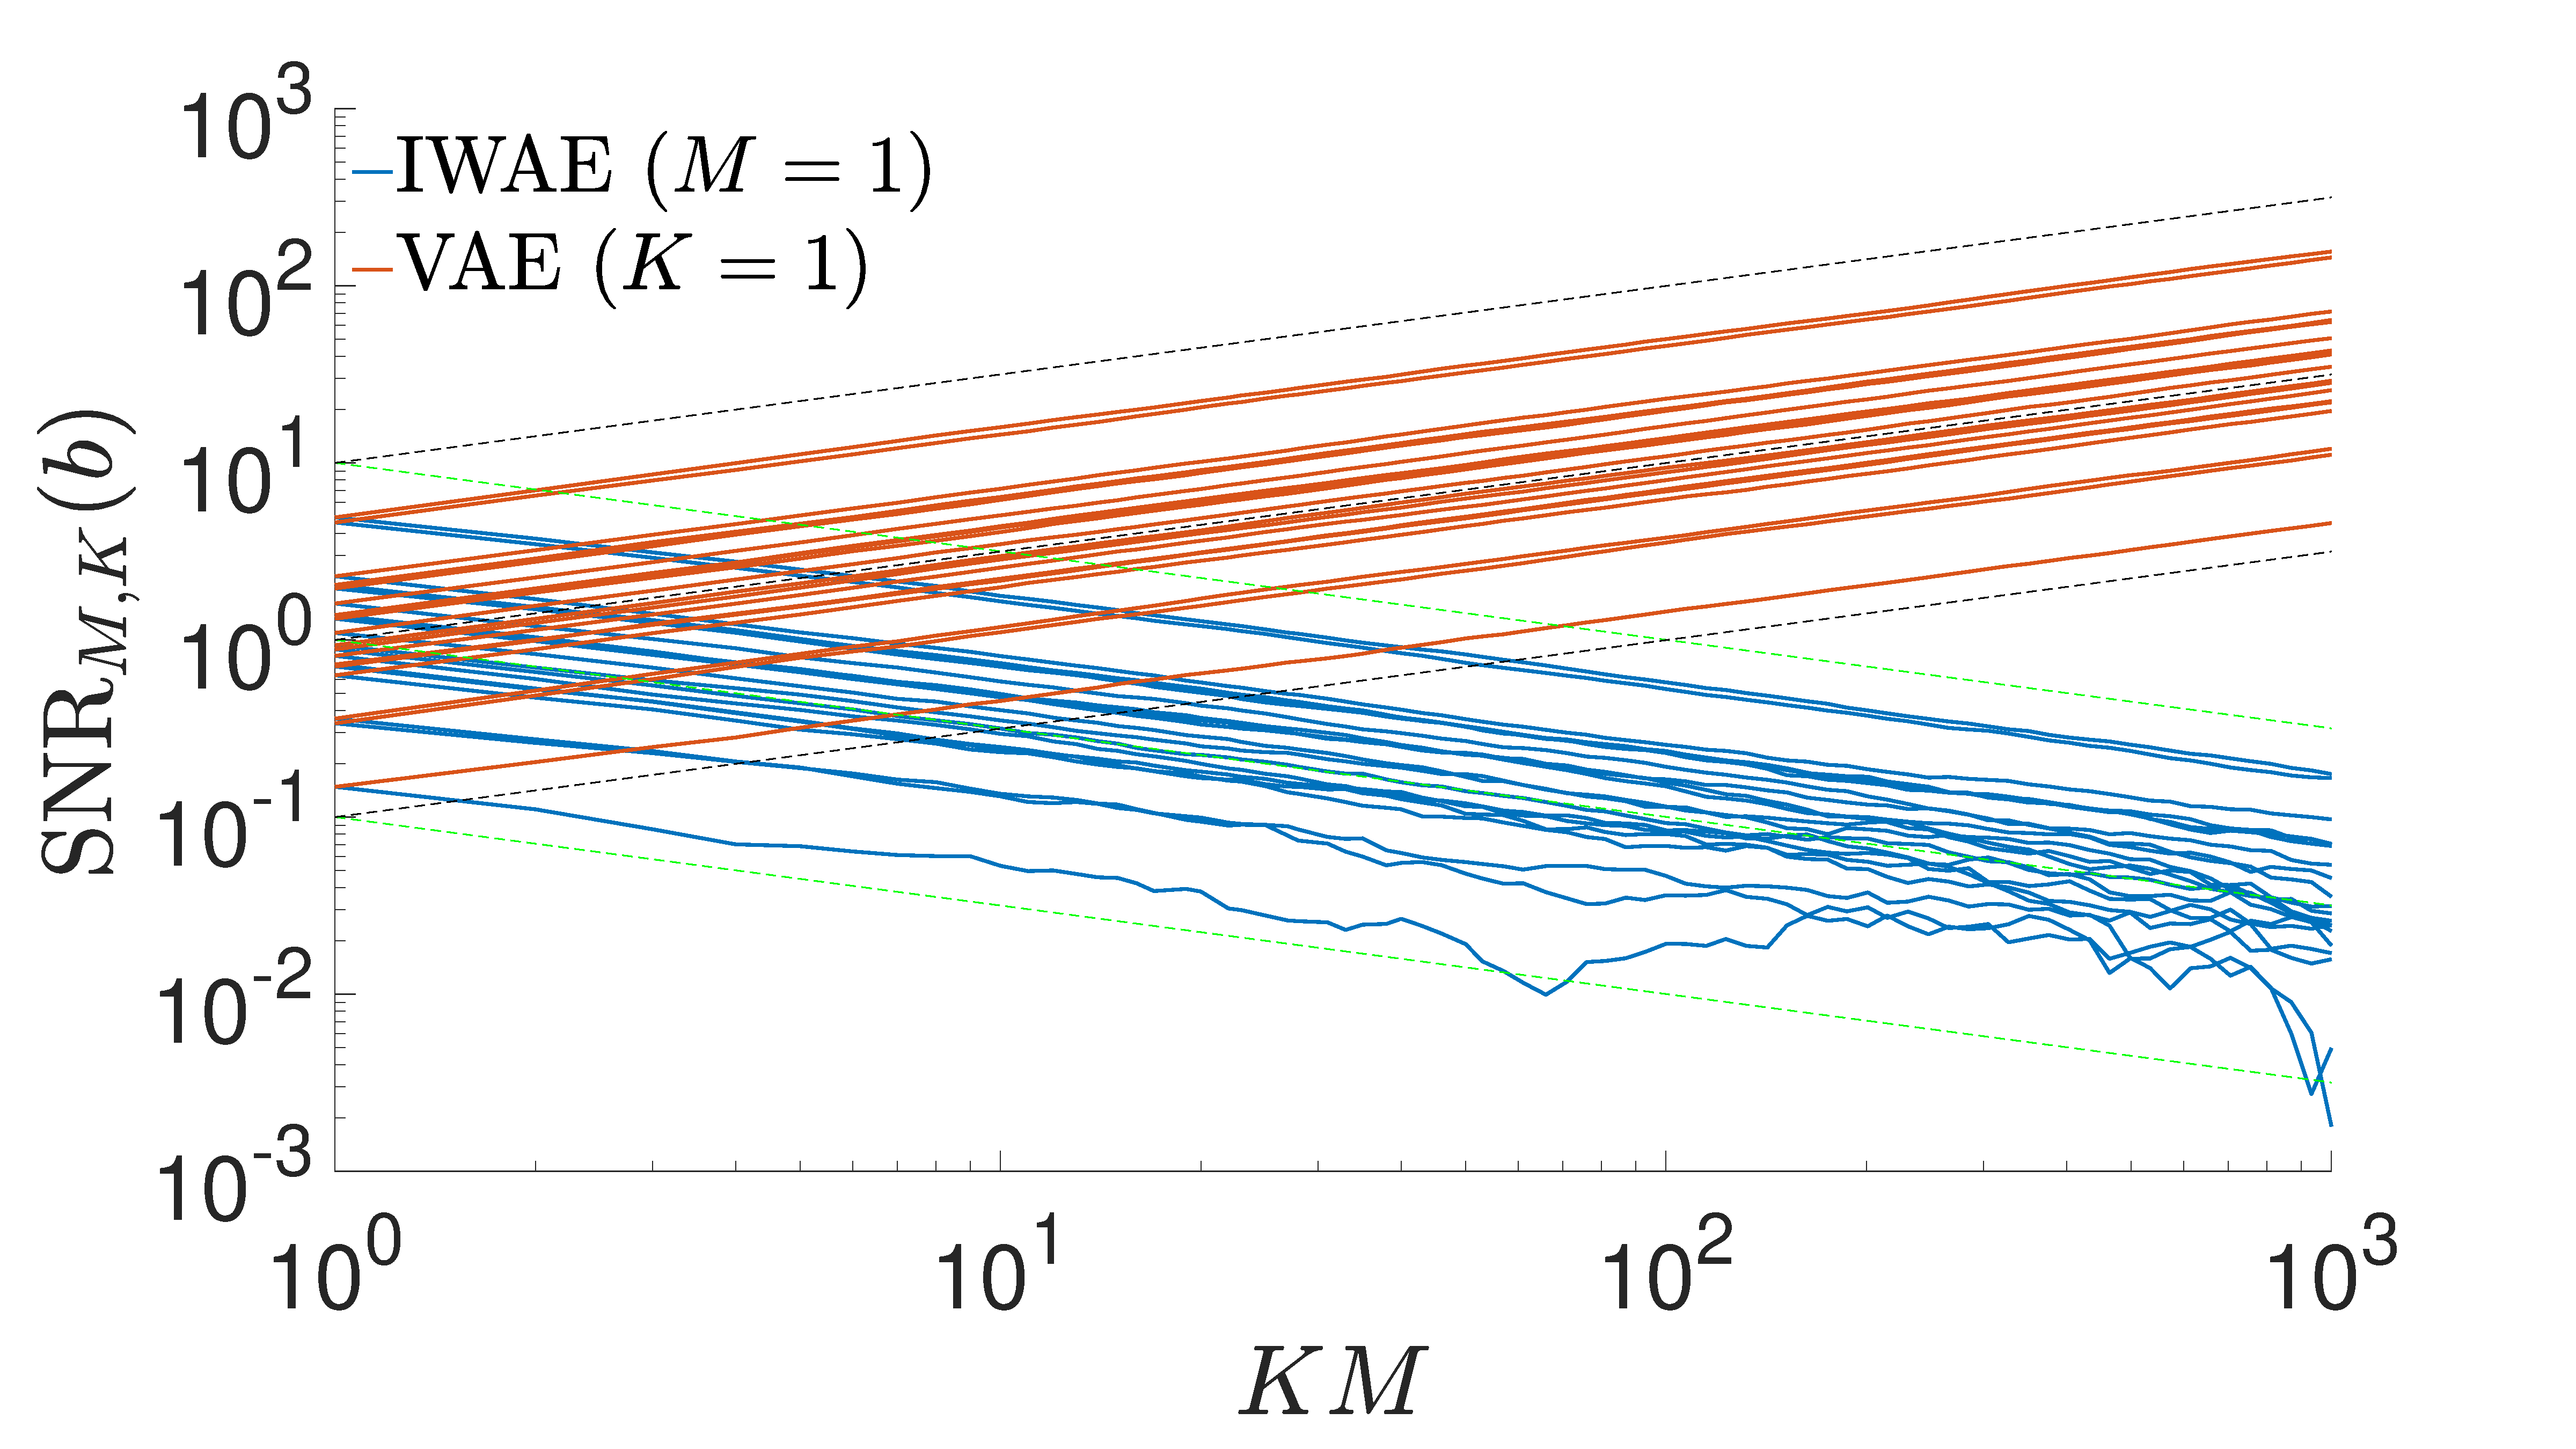
\includegraphics[width=\textwidth]{figures/tighter_bounds/b_conv}
		\caption{Convergence of \gls{SNR} for inference network \label{fig:snr/b}}
	\end{subfigure}
%	\hfill
	\begin{subfigure}[b]{0.4\textwidth}
		\centering
		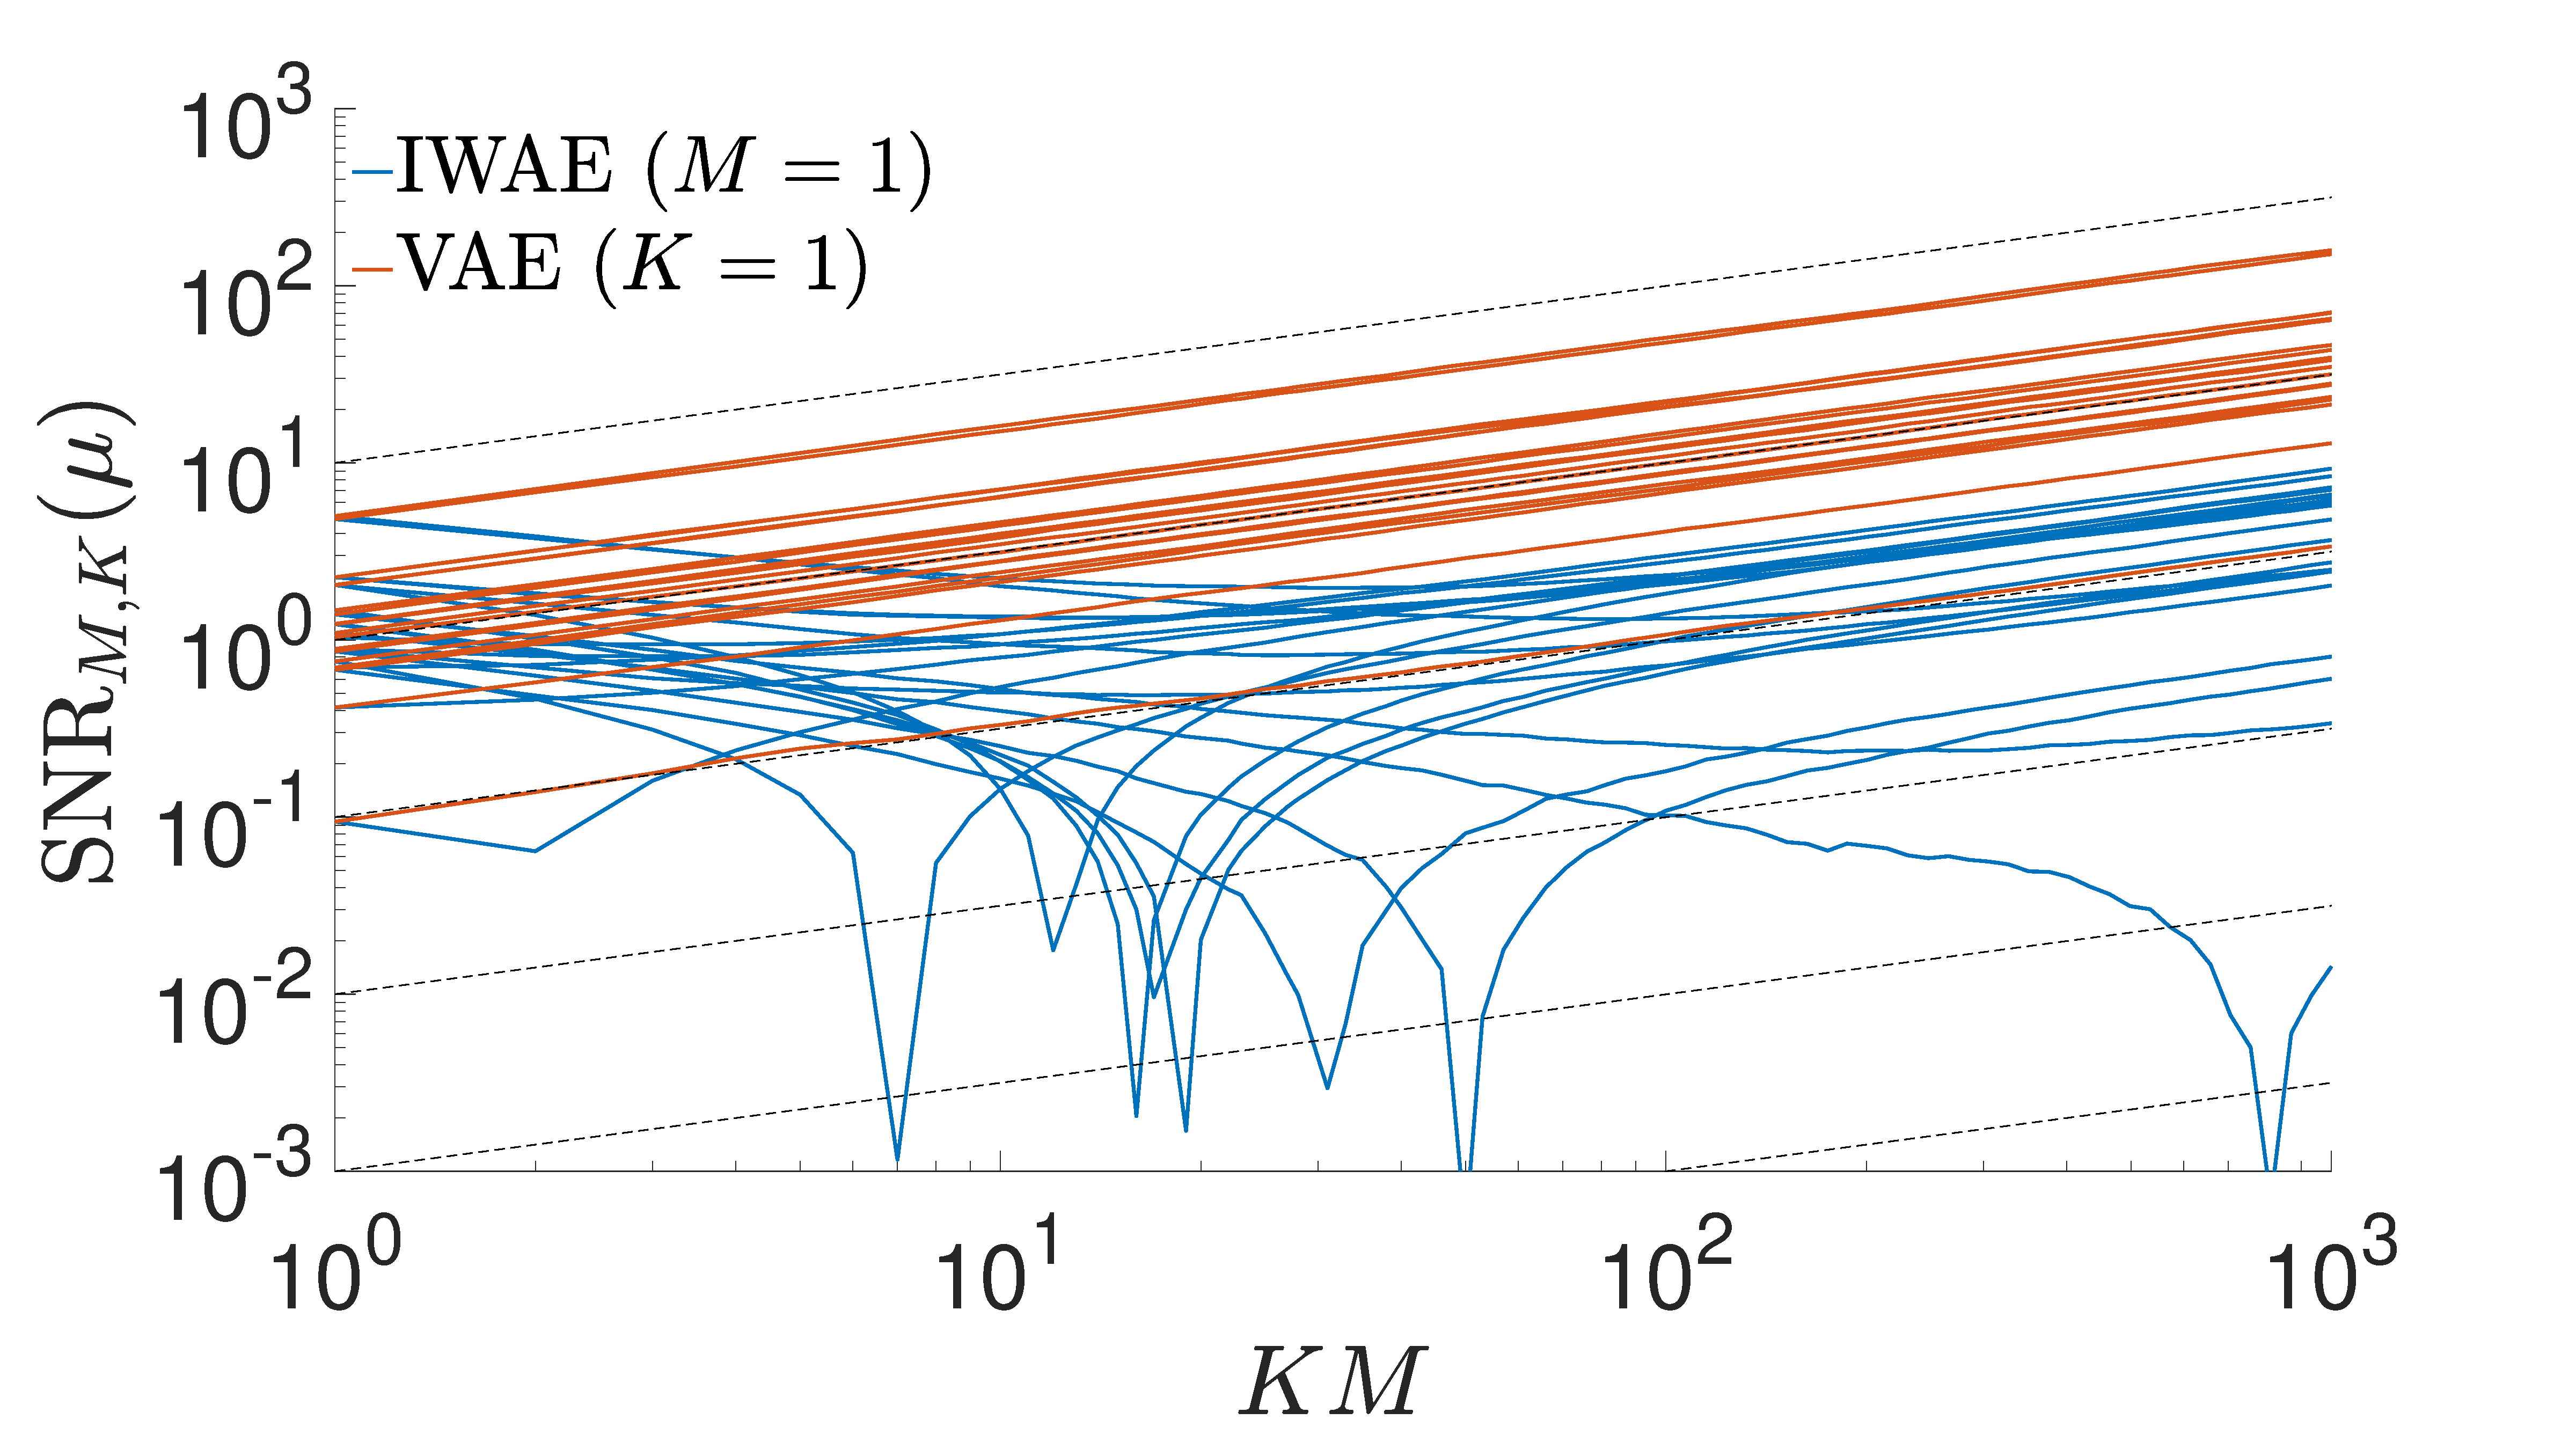
\includegraphics[width=\textwidth]{figures/tighter_bounds/mu_conv}
		\caption{Convergence of \gls{SNR} for generative network\label{fig:snr/mu}}
	\end{subfigure}
	\caption{Convergence of signal-to-noise ratios of gradient estimates with increasing $M$ and $K$.
		Different lines correspond to different
		dimensions of the parameter vectors.
		Shown in blue is the \gls{IWAE} where we keep $M=1$ fixed and increase $K$.  
		Shown in red is the \gls{VAE} where $K=1$ is fixed and we increase $M$. 
		The black and green dashed lines show the expected convergence rates from our theoretical results, 
		representing gradients of $1/2$ and $-1/2$ respectively.  
		\label{fig:snr/K_conv}}
\end{figure*}

To conduct our investigation, we randomly generated a synthetic dataset from the model with $D=20$
dimensions, $N=1024$ data points, and a true model parameter value $\mu_{\text{true}}$ that was itself 
randomly generated from a unit Gaussian, i.e. $\mu_{\text{true}} \sim \mathcal{N}(\mu_{\text{true}} ;0,I)$.
We then considered the gradient at a random point in the parameter space close to optimum (we also 
	consider a point far from the optimum in 
	Appendix~\ref{sec:hv}). Namely
each dimension of each parameter was randomly offset from its optimum value using a zero-mean
Gaussian with standard deviation $0.01$.  We then calculated empirical estimates of the \gls{ELBO}
gradients for \gls{IWAE}, where $M=1$ is held fixed and we increase $K$, and
for \gls{VAE}, where $K=1$ is held fixed and we increase $M$.  In all cases we 
calculated $10^4$ such estimates and used these samples to provide empirical estimates for, amongst other things, the
mean and standard deviation of the estimator, and thereby an empirical estimate for the \gls{SNR}.
%For the inference network, we predominantly focused on investigating the gradients of $b$.

We start by examining the qualitative behavior of the different gradient estimators as $K$ increases as
shown in Figure~\ref{fig:snr/hists}.  This shows histograms of the \gls{IWAE}  gradient estimators
for a single parameter of the inference network (left) and generative network (right).
%We see that,
%as expected, the expectation of the gradients does not change with $M$:
%the only effect of increasing $M$ is to
%reduce the variance.  The effect of increasing $K$ is quite different.
We first see in Figure~\ref{fig:snr/b_hist_iwae} that as $K$ increases, both the magnitude and the standard
deviation of the estimator decrease for the inference network, 
with the former decreasing faster.  This
matches the qualitative behavior of our theoretical result, with the \gls{SNR} ratio 
diminishing as $K$ increases.
In particular, the probability that the gradient is positive or negative 
becomes roughly equal for larger
values of $K$, meaning the optimizer is equally likely to increase as decrease the 
inference network parameters at the next iteration.
By contrast, for the generative network, \gls{IWAE} converges towards a 
non-zero gradient, such that,
even though the \gls{SNR} initially decreases with $K$, it then rises again, with a very
clear gradient signal for $K=1000$.


To provide a more rigorous analysis, we next directly examine the convergence of 
the \gls{SNR}.
Figure~\ref{fig:snr/K_conv} shows the convergence of the estimators with increasing $M$ and $K$.
The observed rates for the inference network (Figure~\ref{fig:snr/b})
correspond to our theoretical results, with
the suggested rates observed all the way back to $K=M=1$.  As expected, we see 
that as $M$ increases, so does $\SNR_{M,K}(b)$, but as $K$ increases, $\SNR_{M,K}(b)$ reduces.
%We thus find that in this scenario, $K$ should be kept as low as possible and
%our computational budget should be focused exclusively on increasing $M$ (ignoring the fact
%that we can also vary the number of epochs etc instead).

In Figure~\ref{fig:snr/mu}, we see that
the theoretical convergence for $\SNR_{M,K}(\mu)$
is again observed exactly for variations in $M$, 
but a more unusual behavior is seen for variations in $K$,
where the \gls{SNR} initially decreases before starting to increase again for large enough $K$, 
eventually exhibiting behavior consistent with the theoretical result for large enough $K$.
The driving factor for this is that here
$\E [\Delta_{M,\infty}(\mu)]$  has a smaller magnitude than (and opposite sign to)
$\E [\Delta_{M,1}(\mu)]$  (see Figure~\ref{fig:snr/mu_hist_iwae}).  If we think of the estimators
for all values of $K$ as biased estimates for
$\E [\Delta_{M,\infty}(\mu)]$, we see from our theoretical results that this bias decreases faster 
than the standard deviation.  Consequently, while the magnitude of this bias remains large compared to
$\E [\Delta_{M,\infty}(\mu)]$, it is the predominant component in the true gradient and
we see similar \gls{SNR} behavior as in the inference network.

% $\SNR_{M,\infty}(\mu)$ typically has a smaller magnitude (and often opposite sign)
% to $\SNR_{M,1}(\mu)$.
Note that this does not mean that the 
estimates are getting worse for the generative network.
As we increase $K$ our bound is getting tighter and our estimates closer to
the true gradient for the target that we 
actually want to optimize $\nabla_{\mu} \log Z$.  See 
Appendix~\ref{sec:app:rmse} for more details.
As we previously discussed, it is also the case that increasing $K$ could be beneficial for the inference network
even if it reduces the \gls{SNR} by improving the direction of the expected gradient.
However, as we will now show, the \gls{SNR} is, for this problem,
%we will return to consider a metric that examines this
%direction in Figure~\ref{fig:snr/extra_end}, where we will see that the \gls{SNR} seems to be 
the dominant effect for the inference network.
%The question of what the optimal target is for updating the inference network 
%is somewhat more subjective than for the generative network,
%even if we presume we can
%evaluate the gradients exactly.  We know that
%the optimum is the same if the family of $q_{\phi}$ contains the posterior, but this may not always be
%the case, while the optimization surface may vary away from the optimum.  We leave investigation of
%this question for future work.  

\begin{figure*}[t]
	\centering
	\begin{subfigure}[b]{0.4\textwidth}
		\centering
		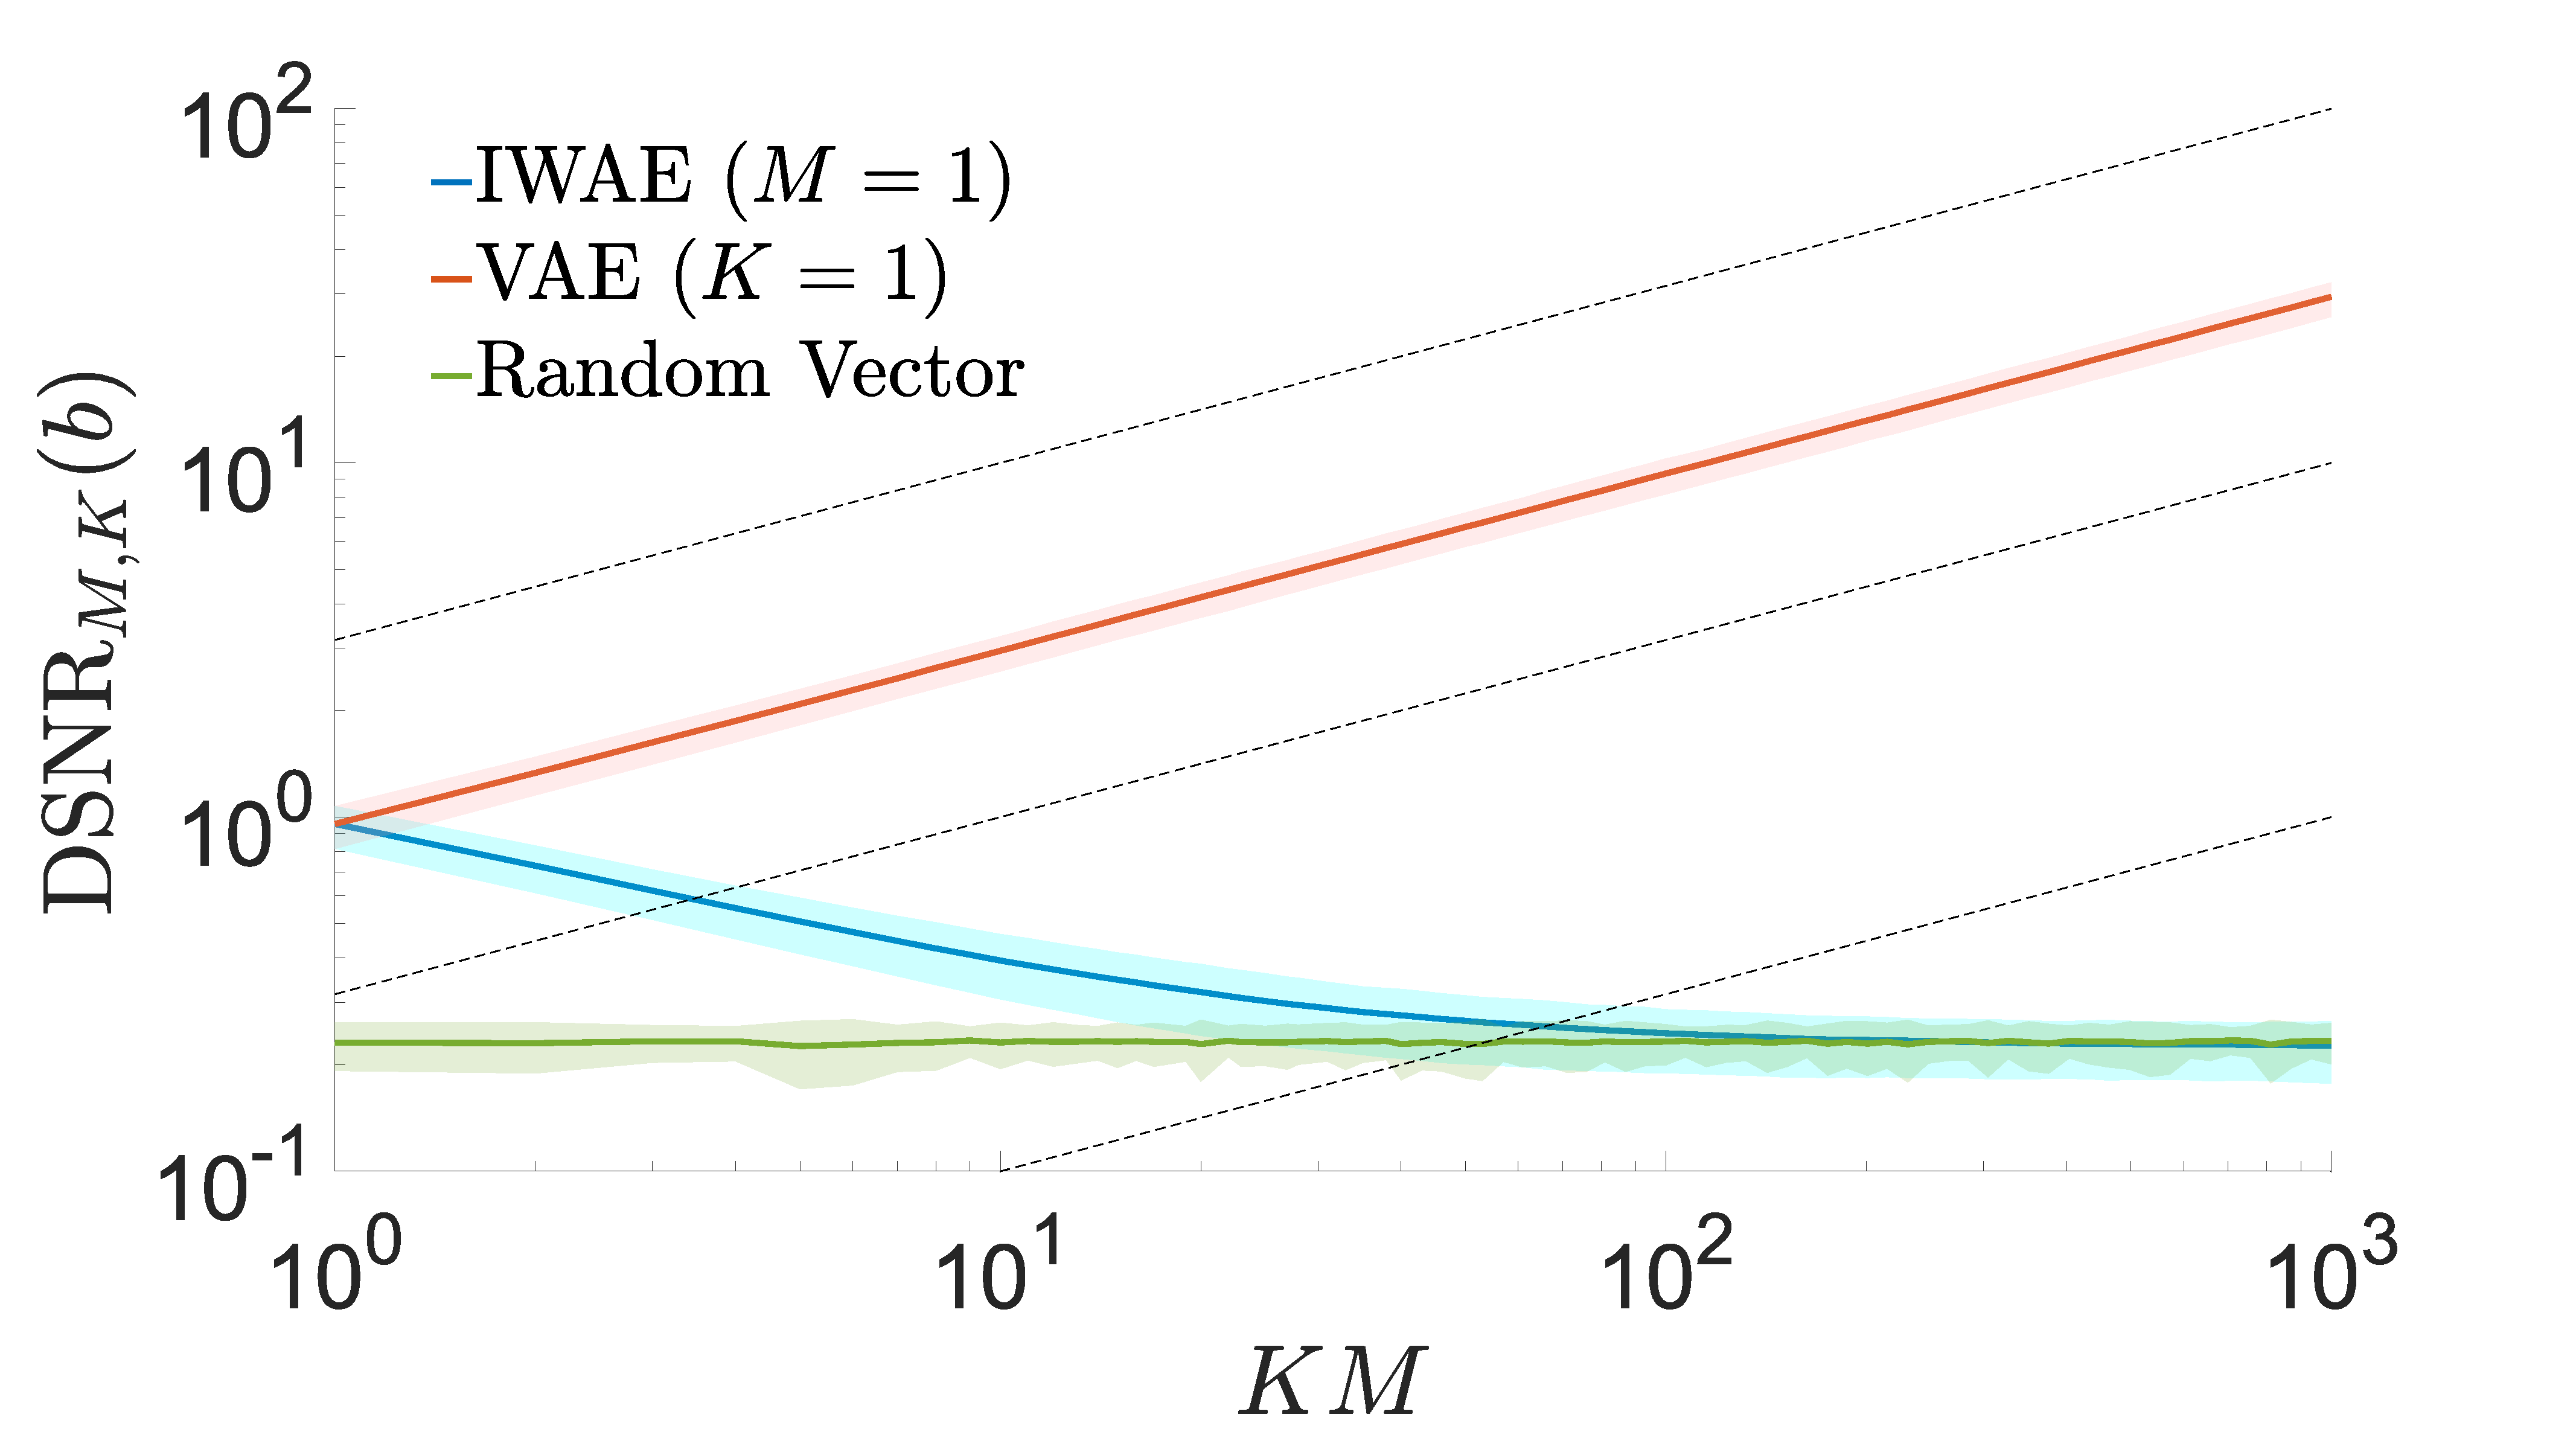
\includegraphics[width=\textwidth]{figures/tighter_bounds/snr_dir}
		\caption{Convergence of \textsc{dsnr} for inference network\label{fig:snr/snr_dir}}
	\end{subfigure}
~~~~~~~~~~~~~~
	\begin{subfigure}[b]{0.4\textwidth}
		\centering
		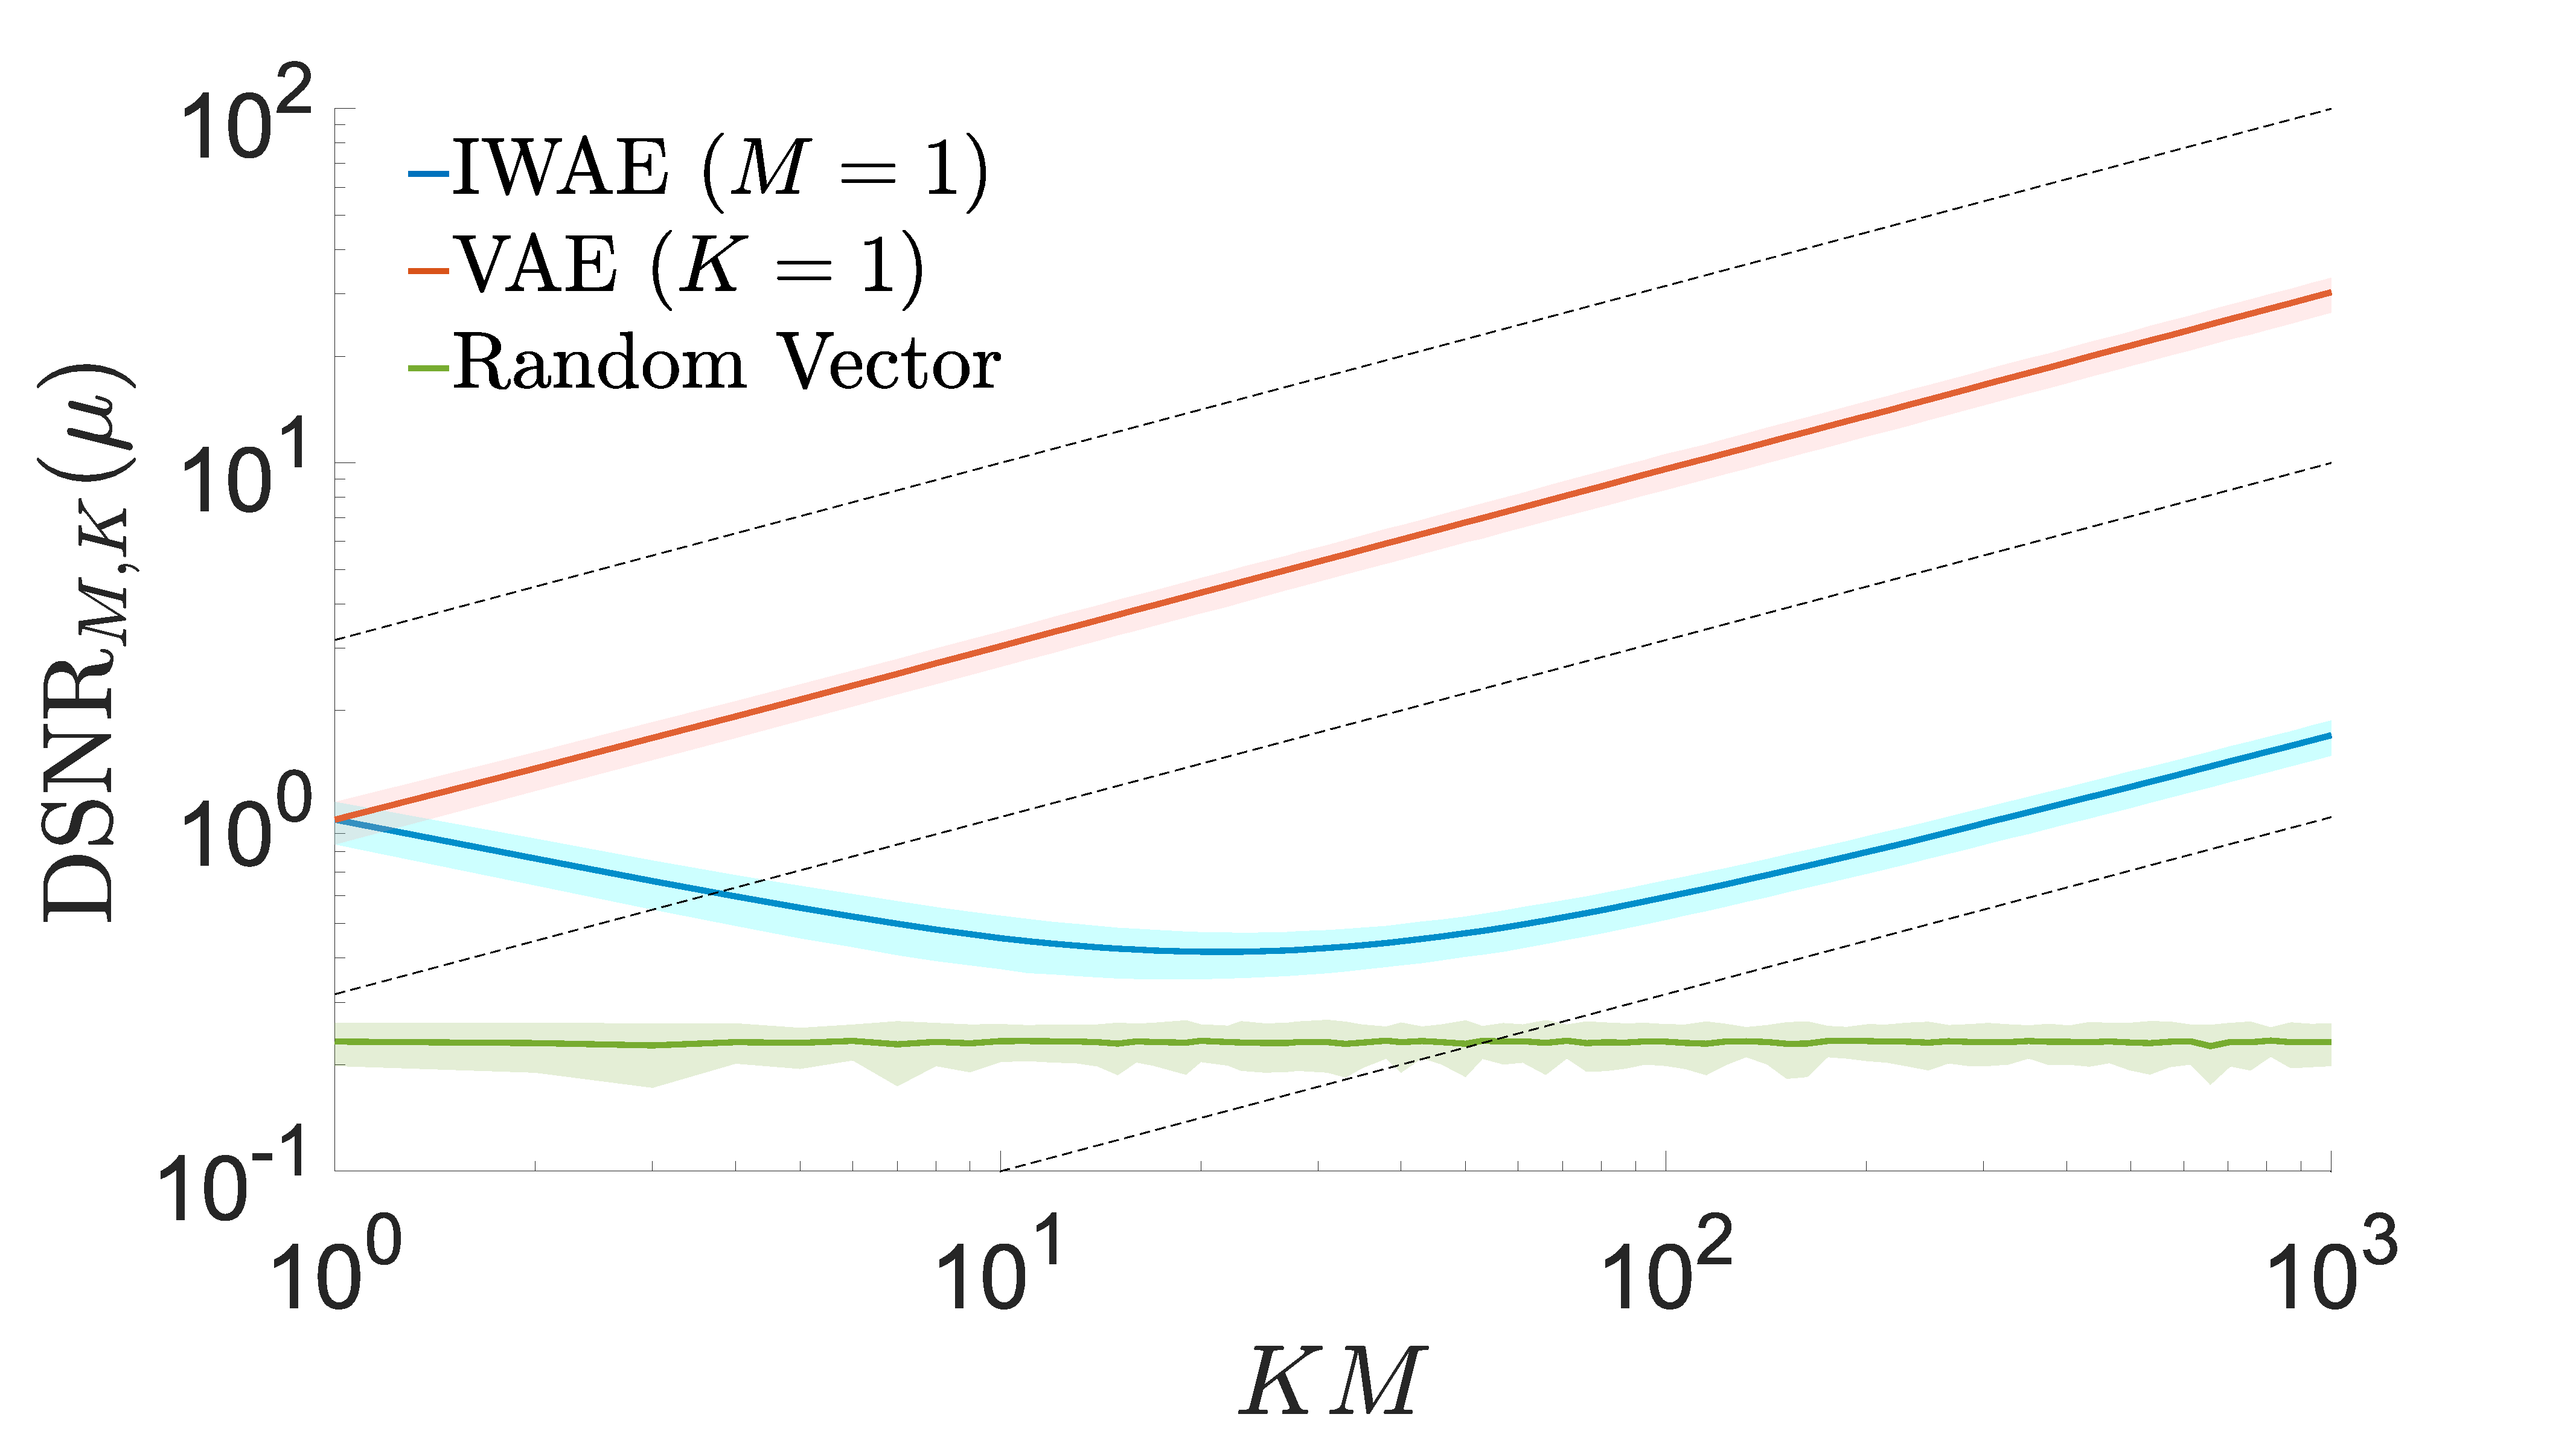
\includegraphics[width=\textwidth]{figures/tighter_bounds/snr_dir_mu}
		\caption{Convergence of \textsc{dsnr} for generative network\label{fig:snr/snr_dir_mu}}
	\end{subfigure}\vspace{-6pt}
	\caption{Convergence of the directional \gls{SNR} of gradients estimates with increasing $M$ and $K$.
		The solid lines show the estimated \textsc{dsnr} and the shaded regions the interquartile range of
		the individual ratios.  Also shown for reference is the \textsc{dsnr} for a randomly generated
		vector where each component is drawn from a unit Gaussian.
		\vspace{-10pt}
		\label{fig:snr/extra}}
\end{figure*}

\begin{figure*}[t]
	\centering
	\begin{subfigure}[b]{0.4\textwidth}
		\centering
		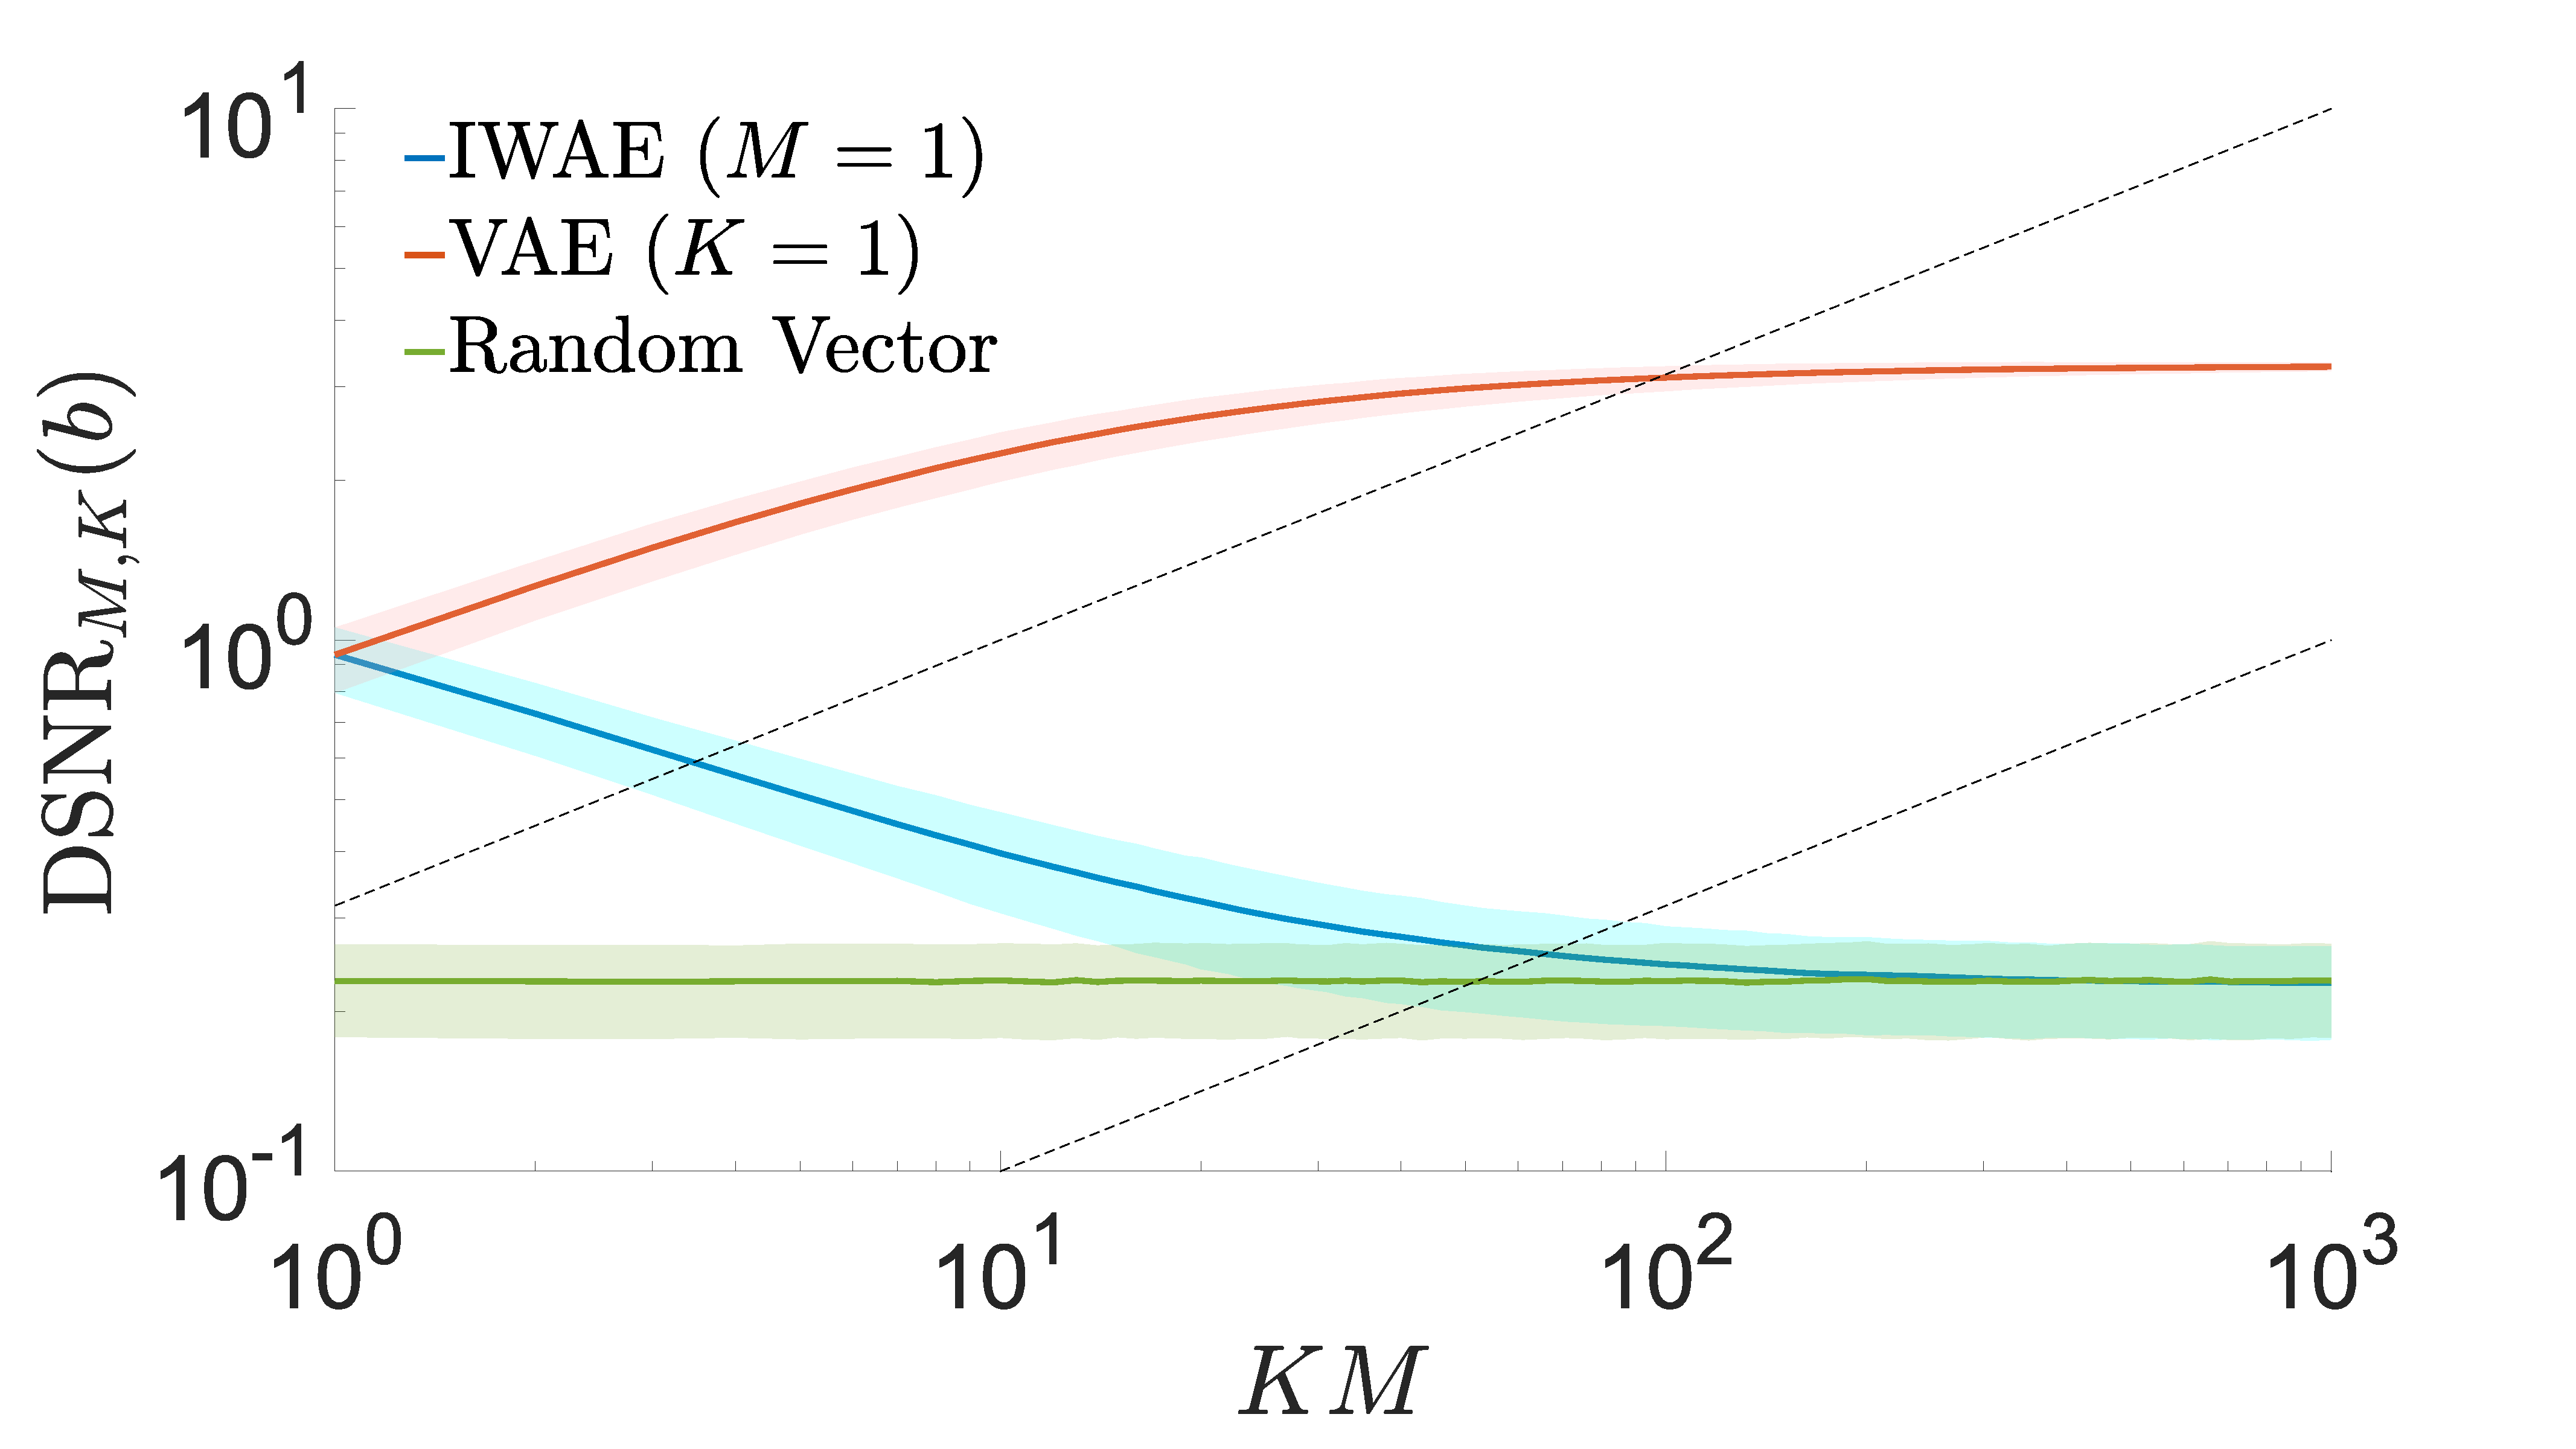
\includegraphics[width=\textwidth]{figures/tighter_bounds/dir_snr_end}
		\caption{Convergence of \textsc{dsnr} for inference network\label{fig:snr/snr_dir_end}}
	\end{subfigure} ~~~~~~~~~~~~~~
	\begin{subfigure}[b]{0.4\textwidth}
		\centering
		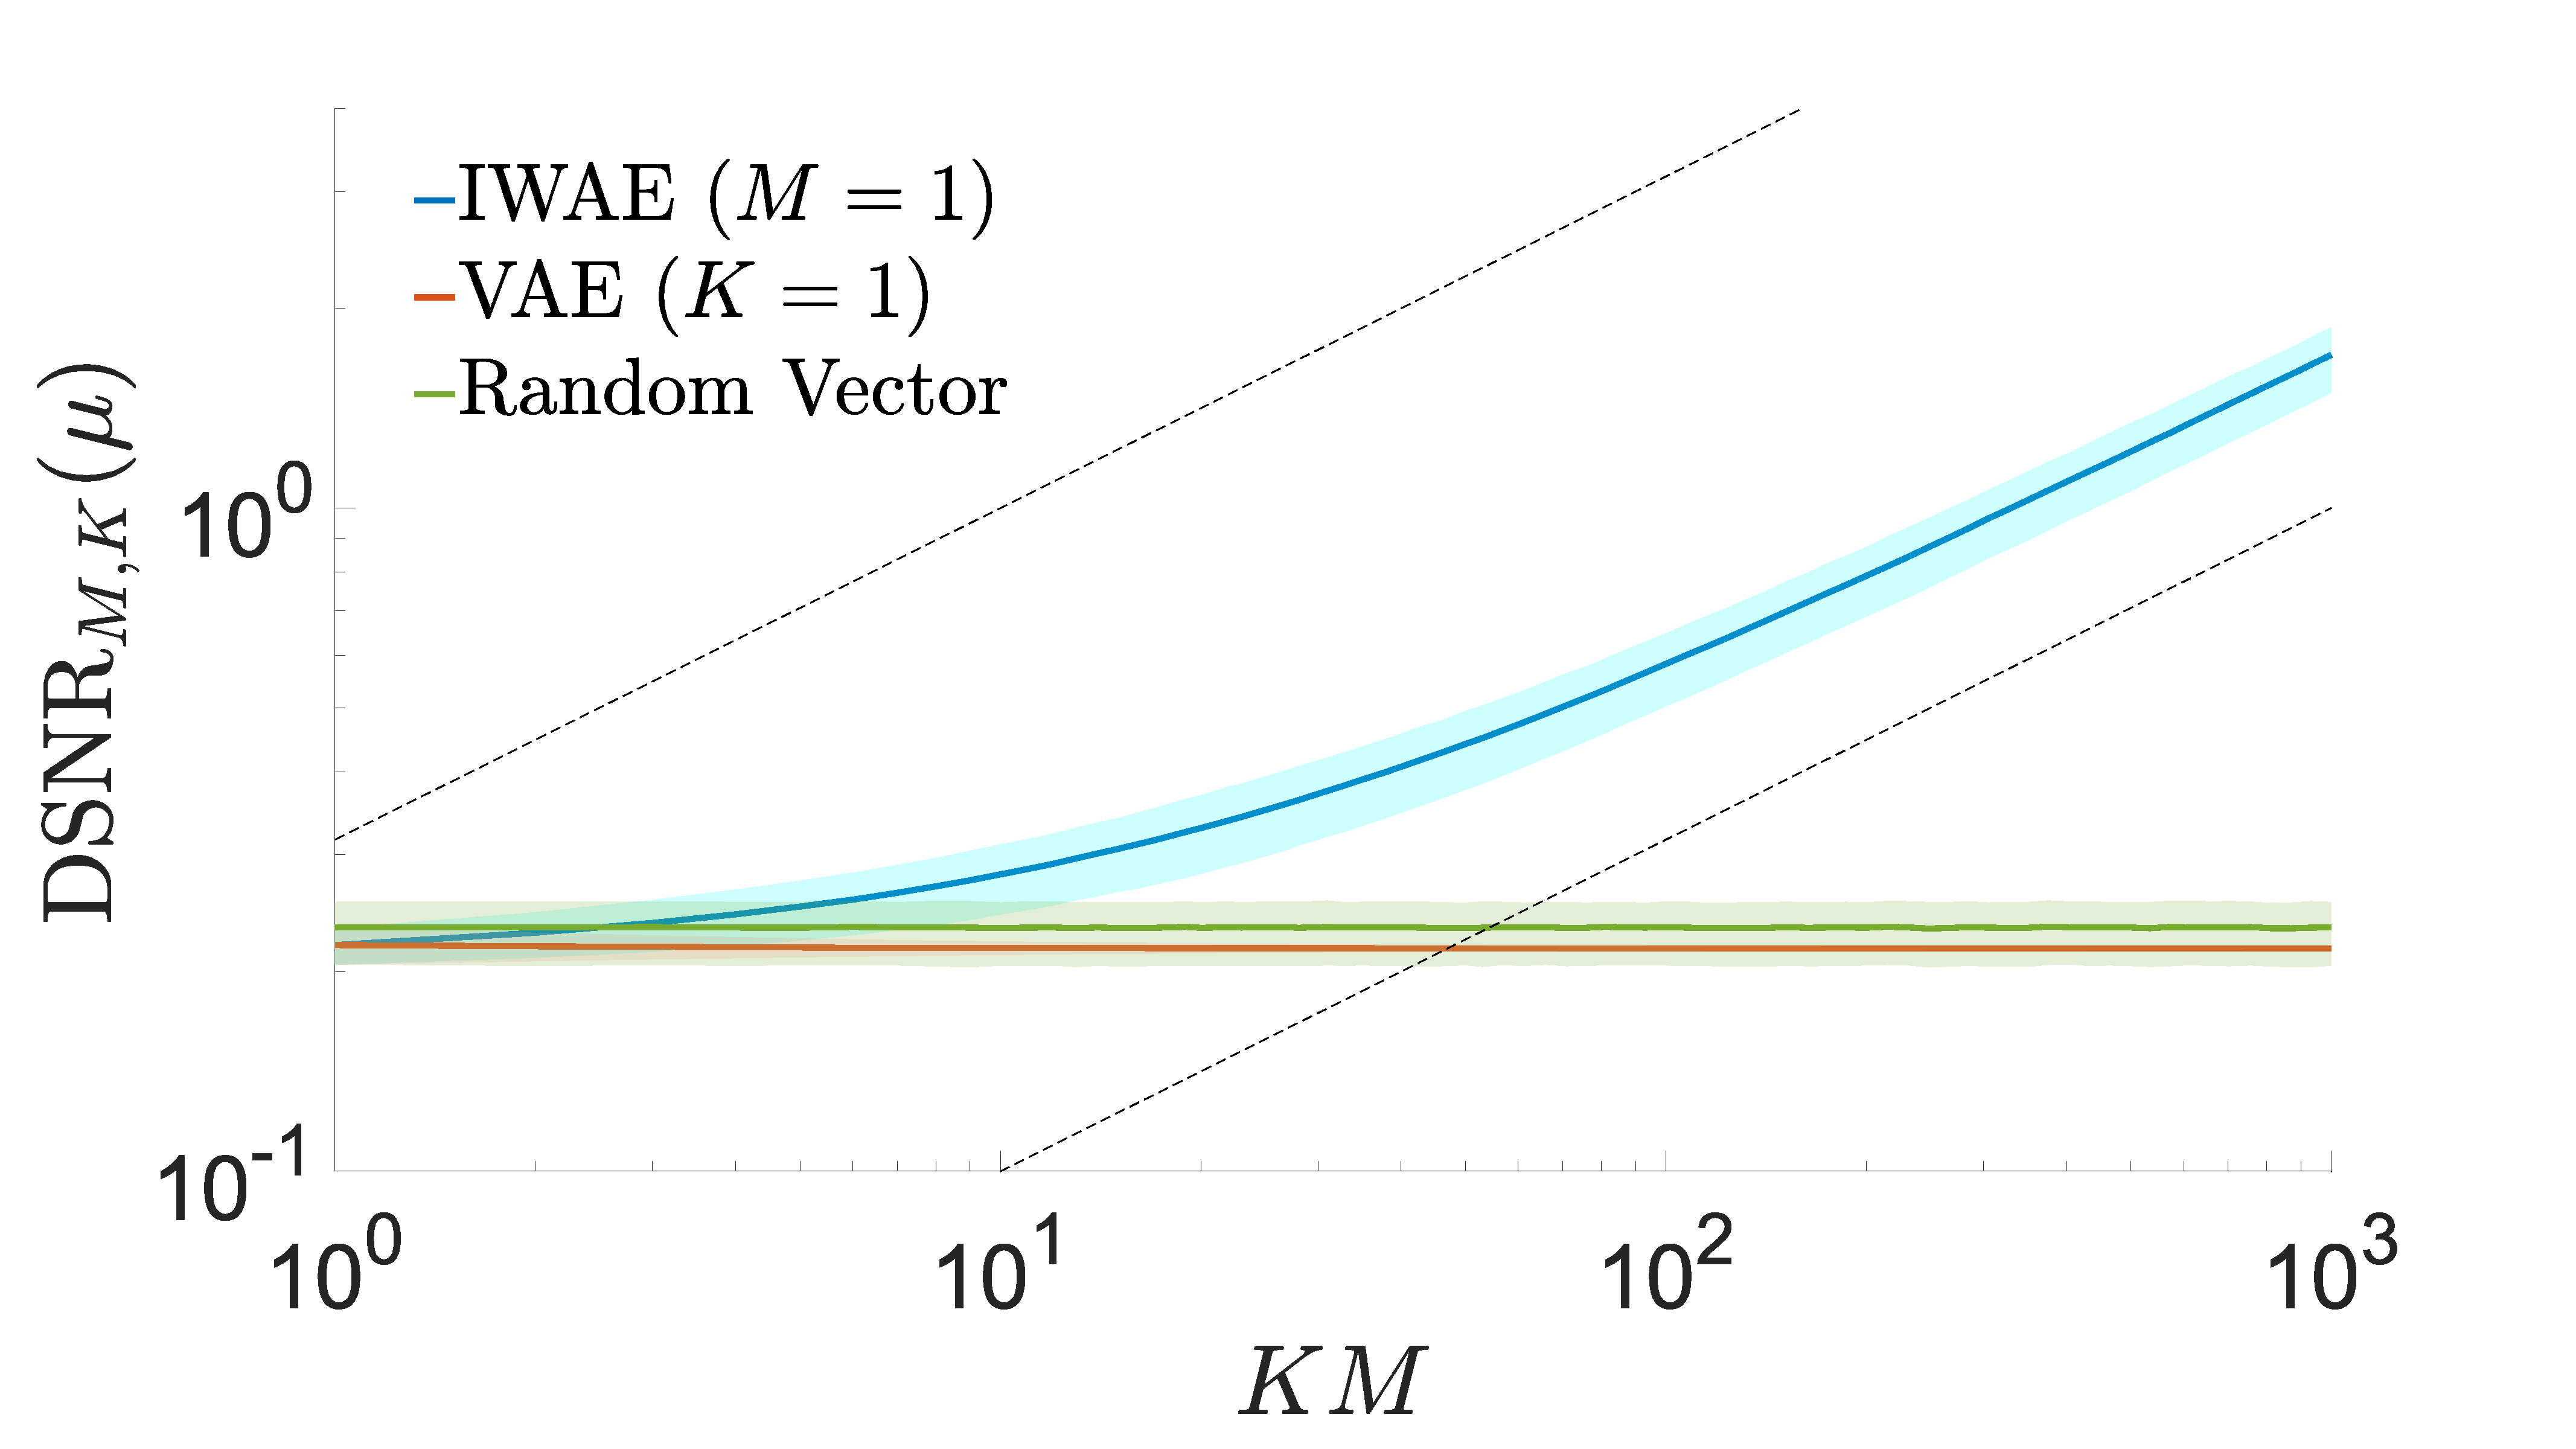
\includegraphics[width=\textwidth]{figures/tighter_bounds/dir_snr_mu_end}
		\caption{Convergence of \textsc{dsnr} for generative network\label{fig:snr/snr_dir_mu_end}}
	\end{subfigure}
	\caption{Convergence of the \textsc{dsnr} when the
		target gradient is taken as $u = \E \left[\Delta_{1,1000}\right]$.  Conventions as
		per Figure~\ref{fig:snr/extra}.
		\label{fig:snr/extra_end}}
\end{figure*}


\subsection{Directional Signal-to-Noise Ratio}

As a reassurance that our chosen definition of the \gls{SNR} is appropriate
for the problem at hand and to examine the effect of multiple dimensions explicitly,
 we now also consider an alternative definition of the \gls{SNR} that is similar (though distinct)
to that used in~\cite{Roberts2009signal}.  We refer to this as the ``directional'' \gls{SNR} (\textsc{dsnr}).
At a high-level, we define the \textsc{dsnr} by splitting each gradient estimate into two component vectors, one parallel
to the true gradient and one perpendicular, then taking the expectation of ratio of their magnitudes.  More precisely,
we define $u =\E \left[\Delta_{M,K}\right]/\lVert\E \left[\Delta_{M,K}\right]\rVert_2$ as being
the true normalized gradient direction and then the \textsc{dsnr} as
\begin{align}
\textsc{dsnr}_{M,K} = & \,\,\E \left[\frac{\lVert\Delta_{\|}\rVert_2}{\lVert\Delta_{\bot}\rVert_2} \right]
\quad \text{where}  \displaybreak[0]\\
\Delta_{\|} = \left(\Delta_{M,K}^T u\right)u &\quad \text{and} \quad
\Delta_{\bot} = \Delta_{M,K}- \Delta_{\|}. \nonumber
\end{align}
The \textsc{dsnr} thus provides a measure of the expected proportion of the gradient that will point in the
true direction.  For perfect estimates of the gradients, then $\textsc{dsnr}\to\infty$, but unlike the
\gls{SNR}, arbitrarily bad estimates do not have $\textsc{dsnr}=0$ because even random vectors will have
a component of their gradient in the true direction.

The convergence of the \textsc{dsnr} is shown in Figure~\ref{fig:snr/extra}, for which the true normalized
gradient $u$ has been estimated empirically, noting that this varies with $K$.
We see a similar qualitative behavior
to the \gls{SNR}, with the gradients of \gls{IWAE} for the inference network degrading to having the
same directional accuracy as drawing a random vector.  Interestingly, the \textsc{dsnr} seems to be
following the same asymptotic convergence behavior as the \gls{SNR} for both
networks in $M$ (as shown by the dashed lines), even though we have no theoretical result to suggest this should occur.



As our theoretical results suggest that the direction of the true gradients correspond to
targeting an improved objective 
as $K$ increases, we now examine whether this or the changes in
the \gls{SNR} is the dominant effect.  To this end, we repeat our calculations for
the \textsc{dsnr} but take $u$ as the target direction of the gradient for $K=1000$. 
This provides a measure of how varying $M$ and $K$ affects the quality of the gradient directions
as biased estimators for $\E\left[\Delta_{1,1000}\right]
/\lVert\E\left[\Delta_{1,1000}\right]\rVert_2$.  As shown in Figure~\ref{fig:snr/extra_end}, increasing $K$ is still detrimental for the inference network
by this metric, even though
it brings the expected gradient estimate closer to the target gradient.  By contrast, increasing
$K$ is now monotonically beneficial for the generative network.  Increasing $M$
leads to initial improvements for the inference network before plateauing due to the bias 
of the estimator.  For the generative network, increasing $M$ has little impact, with the bias being
the dominant factor throughout.  Though this metric is not an absolute measure of
performance of the~\gls{SGA} scheme, e.g. because high bias may be more detrimental than high variance,
it is nonetheless a powerful result in suggesting that increasing $K$ can be detrimental
to learning the inference network.



% !tex root=./main.tex

\section{Discussion}
\label{sec:discussion}

The central argument here is that where one needs both amortization and model learning for \glspl{SCFM}, the \gls{RWS} family of methods is preferable to \gls{IWAE} with either continuous relaxations or control-variates.
%
The \gls{PCFG} experiment (\cref{sec:experiments/pcfg}) demonstrates a setting where continuous relaxations are inapplicable due to potentially infinite recursion, but where \gls{RWS} applies and \gls{WS} outperforms all other methods.
%
The \gls{AIR} experiment (\cref{sec:experiments/air}) highlights a case where with more particles, performance of \gls{VIMCO} degrades for the inference network~\citep{Rainforth2018tighter} and consequently the generative model as well, but where \gls{RWS}'s performance on both increases monotonically.
%
Finally, the analysis on \glspl{GMM} (\cref{sec:experiments/gmm}) focuses on a simple model to understand nuances in the performances of different methods.
%
Beyond implications from prior experiments, it indicates that for the few-particle regime, the \gls{WW} gradient estimator can be biased, leading to poor learning.
%
%
For this, we design an alternative involving defensive sampling that ameliorates the issue.
%
The precise choice of which variant of \gls{RWS} to employ depends on which of the two kinds of gradient bias described in \cref{sec:disadvantages} dominates.
%
Where the data distribution bias dominates, as with the \gls{AIR} experiment, \gls{WW} is preferable, and where the self-normalized \gls{IS} bias dominates, as in the \gls{PCFG} experiment, \gls{WS} is preferable.
In the \gls{GMM} experiment, we verify this empirically by studying two optimization procedures with low and high data distribution biases.

%%% Local Variables:
%%% mode: latex
%%% TeX-master: "main"
%%% End:

%  LocalWords:  SCFM RWS IWAE variates PCFG WS VIMCO rainforth GMM


\subsubsection*{Acknowledgments}

TAL's research leading to these results is supported by EPSRC DTA and Google (project code DF6700) studentships.
AK's and YWT's research leading to these results are supported by funding from the European Research Council under the European Union’s Seventh Framework Programme (FP7/2007-2013) ERC grant agreement no. 617071.
NS is supported by EPSRC/MURI grant EP/N019474/1.
FW's research leading is supported by The Alan Turing Institute under the EPSRC grant EP/N510129/1; DARPA PPAML through the U.S. AFRL under Cooperative Agreement FA8750-14-2-0006; Intel and DARPA D3M, under Cooperative Agreement FA8750-17-2-0093.

\clearpage
\newpage

\renewcommand*{\bibfont}{\small}
\bibliography{main}
\bibliographystyle{plainnat}
\balance

\clearpage
\newpage
\appendix
% !tex root=./main.tex

\section{PROBABILISTIC CONTEXT-FREE GRAMMAR}
\label{app:pcfg}

We show the \emph{astronomers} \gls{PCFG} in \cref{fig:app/pcfg/astronomers}.
\Cref{fig:experiments/pcfg/vimco_q_samples} shows samples from an inference network trained with \gls{VIMCO} with $K = 20$, conditioned on the sentence $x = $ ``astronomers saw stars with telescopes''.
\Cref{fig:experiments/pcfg/production_probs} shows production probabilities of the non-terminal NP learned by \gls{VIMCO} and \gls{WS} with $K = 20$.
\begin{figure}[htb]
  \begin{align*}
    \text{S} \to&\,\, \text{NP}\,\text{VP}\,(1.0) \\
    \text{NP} \to&\,\, \text{NP}\,\text{PP}\,(0.4) | \text{astronomers}\,(0.1) | \text{ears}\,(0.18) | \\
    &\,\, \text{saw}\,(0.04) | \text{stars}\,(0.18) | \text{telescopes}\,(0.1) \\
    \text{VP} \to&\,\, \text{V}\,\text{NP}\,(0.7) | \text{VP}\,\text{PP}\,(0.3) \\
    \text{PP} \to&\,\, \text{P}\,\text{NP}\,(1.0) \\
    \text{P} \to&\,\, \text{with}\,(1.0) \\
    \text{V} \to&\,\, \text{saw}\,(1.0).
  \end{align*}
  \caption{\emph{The astronomers \acrshort{PCFG}} from \citet[Table 11.2]{manning1999foundations}. The terminals are $\{\text{astronomers}, \text{ears}, \text{saw}, \text{stars}, \text{telescopes}, \text{with}\}$, the non-terminals are $\{\text{S}, \text{NP}, \text{VP}, \text{PP}, \text{P}, \text{V}\}$ and the start symbol is S.
  Each row above lists production rules $\{n_i \to \zeta_j\}$ with the corresponding probabilities $p_{ij}$ in the format $n_i \to \zeta_1\,(p_{i1}) | \zeta_2\,(p_{i2}) | \cdots | \zeta_J\,(p_{iJ})$.}
  \label{fig:app/pcfg/astronomers}
\end{figure}
\begin{figure}[htb]
  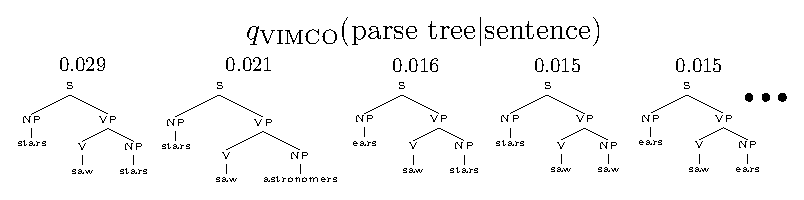
\includegraphics[scale=0.6]{figures/pcfg/vimco_q_samples.eps}
  \caption{Samples from the inference network which was trained with \gls{VIMCO} with $K = 20$.}
  \label{fig:experiments/pcfg/vimco_q_samples}
  \vspace*{-2ex}
\end{figure}
\begin{figure}[htb]
  \centering
  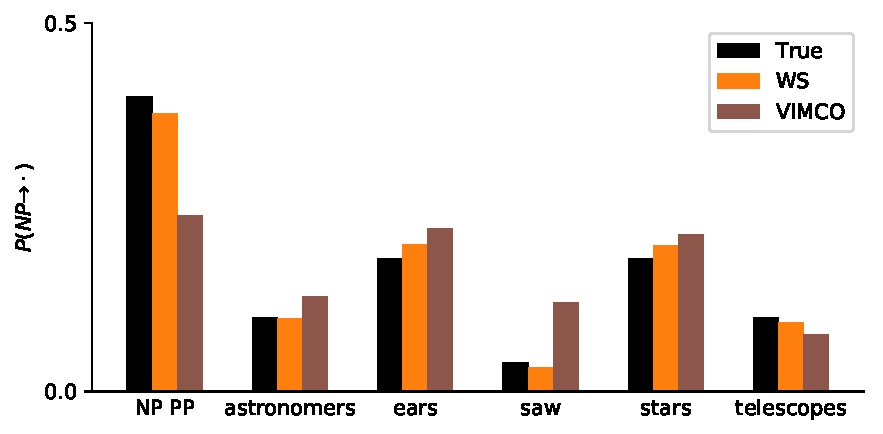
\includegraphics[width=0.7\linewidth]{figures/pcfg/np_probs.pdf}
  \caption{Production probabilities for the non-terminal NP learned via \gls{WS} and \gls{VIMCO} with $K = 20$.}
  \label{fig:experiments/pcfg/production_probs}
  \vspace*{-2ex}
\end{figure}


\section{ATTEND, INFER, REPEAT}
\label{app:air}

\Gls{AIR} is a model with many components and might be difficult to understand if not described explicitly.
Here, we outline details of our implementation and provide pseudo-code for the inference (\cref{algo:air_inference}) and generative models (\cref{algo:air_generation}) in the case of continuous data and Gaussian data likelihood.

\begin{algorithm}[!h]
    \caption{Inference in \gls{AIR}}
    \label{algo:air_inference}
    \DontPrintSemicolon
    % \SetAlgoLined
    \SetKwInOut{Input}{Input}
    \SetKwInOut{Output}{Output}
    \SetSideCommentLeft
    \Input{Image $\bm{x}$,\\ maximum number of inference steps $N$}
    $\bm{h}_0, \bm{z}^\text{what}_0, \bm{z}^\text{where}_0$ = initialize()\\
    \For{$n \in [1, \dots, N]$}{
        $\bm{w}_n, \bm{h}_n = R_\phi \left( \bm{x}, \bm{z}^\text{what}_{n-1}, \bm{z}^\text{where}_{n-1}, \bm{h}_{n-1} \right)$\\
        $p_n \sim \mathrm{Bernoulli} (p \mid \bm{w}_n)$\\
        \If{$p_n = 0$}{
            break
        }
        $\bm{z}^\text{where}_n \sim q_\phi^\text{where} \left( \bm{z}^\text{where} \mid \bm{w}_n \right)$\\
        $\bm{g}_n = \text{STN} \left( \bm{x}, \bm{z}^\text{where}_n \right)$\\
        $\bm{z}^\text{what}_n \sim q_\phi^\text{what} \left( \bm{z}^\text{what} \mid \bm{g}_n \right)$\\
    }
\Output{$\bm{z}^\text{what}_{1:n}$, $\bm{z}^\text{where}_{1:n}$, $n$}
\end{algorithm}
\begin{algorithm}[!h]
    \caption{Generation in \gls{AIR}}
    \label{algo:air_generation}
    \DontPrintSemicolon
    \SetKwInOut{Input}{Input}
    \SetKwInOut{Output}{Output}
    \SetSideCommentLeft
    \Input{$\bm{z}^\text{what}_{1:n}$, $\bm{z}^\text{where}_{1:n}$, $n$}
    $\bm{y}_0 = \bm{0}$\\
    \For{$t \in [1, \dots, n]$}{
        $\hat{\bm{g}}_t = h_\theta^\text{dec} \left( \bm{z}^\text{what}_t \right)$\\
        $\bm{y}_t = \bm{y}_{t-1} + \text{STN}^{-1} \left( \hat{\bm{g}}_t, \bm{z}^\text{where}_t \right)$\\
    }
    $\hat{\bm{x}} \sim \mathrm{Normal} \left(\bm{x} \mid \bm{y}_n, \sigma^2_x \bm{I} \right)$\\
    \Output{$\hat{\bm{x}}$}
\end{algorithm}
\vspace*{-2ex}

\section{GAUSSIAN MIXTURE MODEL}
\label{app:gmm}

\subsection{CONTROL VARIATES}
Here, we present the architectures for the \acrshort{REBAR}/\acrshort{RELAX} control variate used in the \gls{GMM} experiment.

The reparameterized sampling of Gumbels and conditional Gumbels is described by \citet[Appendix C]{tucker2017rebar} and \citet[Appendix B]{grathwohl2018backpropagation}.
In the following, we describe architectures used for the \gls{GMM} experiment (\cref{sec:experiments/gmm}).

\Acrshort{REBAR} proposes the following architecture for the control variate $c_\rho(g_{1:K})$:
\begin{align}
    c_\rho^{\acrshort{REBAR}}(g_{1:K}) = \rho_1 \log\left(\frac{1}{K} \sum_{k = 1}^K \frac{p_\theta(\mathrm{sm}(g_k / e^{\rho_2}), x)}{q_\phi(\mathrm{sm}(g_k / e^{\rho_2}) \given x)}\right), \label{eq:rebar-c}
\end{align}
where $\rho = (\rho_1, \rho_2)$, and $\mathrm{sm}$ refers to the softmax function.
While the functional form of \cref{eq:rebar-c} suggests that it will be highly correlated with $\log(\frac{1}{K} \sum_{k = 1}^K w_k)$, the terms \glspl{PMF} in the fraction are undefined due to the softmax.
A straightforward fix is to evaluate ``a soft \gls{PMF}'' instead:
\begin{align*}
    &p_\theta(\mathrm{sm}(g_k / e^{\rho_2}), x) \\
    &= p_\theta(\mathrm{sm}(g_k / e^{\rho_2})) p(x \given \mathrm{sm}(g_k / e^{\rho_2})) \\
    &= \mathrm{Categorical}(\mathrm{sm}(g_k / e^{\rho_2}) \given \mathrm{sm}(\theta)) \cdot \\
    & \qquad\mathrm{Normal}(x \given \mu_{\mathrm{sm}(g_k / e^{\rho_2})}, \sigma_{\mathrm{sm}(g_k / e^{\rho_2})}^2) \\
    &\approx  \mathrm{sm}(g_k / e^{\rho_2})^\intercal \mathrm{sm}(\theta) \cdot \\
    & \qquad \mathrm{Normal}(x \given \mu^\intercal \mathrm{sm}(g_k / e^{\rho_2}), (\sigma^2)^\intercal \mathrm{sm}(g_k / e^{\rho_2})), \\
    &q_\phi(\mathrm{sm}(g_k / e^{\rho_2}) \given x) \\
    &= \mathrm{Categorical}(\mathrm{sm}(g_k / e^{\rho_2}) \given \mathrm{sm}(\eta_\phi(x))) \\
    &\approx \mathrm{sm}(g_k / e^{\rho_2})^\intercal \mathrm{sm}(\eta_\phi(x)).
\end{align*}
Optimization of the log-temperature $\rho_2$ is highly sensitive as low values can make the training unstable.

\Acrshort{RELAX} proposes using an arbitrary neural network for $c_\rho(g_{1:K})$.
Due to the symmetry in the arguments, we pick the following for the \gls{GMM} experiment:
\begin{align}
    c_\rho^{\acrshort{RELAX}}(g_{1:K}) = \frac{1}{K} \sum_{k = 1}^K \acrshort{MLP}_\rho([x, g_k]), \label{eq:relax-c}
\end{align}
where the architecture of the \gls{MLP} is $(1 + C)$-$16$-$16$-$1$ (with the $\tanh$ nonlinearity between layers) and $\rho$ are the weights are its weights.
This architecture is---unlike the one in \cref{eq:rebar-c}---well-defined for all inputs.
A drawback of using such control variate is that it can start out not being very correlated with $\log(\frac{1}{K} \sum_{k = 1}^K w_k)$.

\Acrshort{RELAX} also proposes using a summation of the free-form control variate like the one in \cref{eq:relax-c} and a more correlated control variate in \cref{eq:rebar-c}.

We have tried all architectures and found that \cref{eq:relax-c} leads to the most stable and best training.

Using \acrshort{REBAR}/\acrshort{RELAX} for more complicated models is possible, however designing an architecture that is highly correlated with the high-variance term and stable to train still remains a challenge.

\begin{figure*}[!htb]
  \centering
  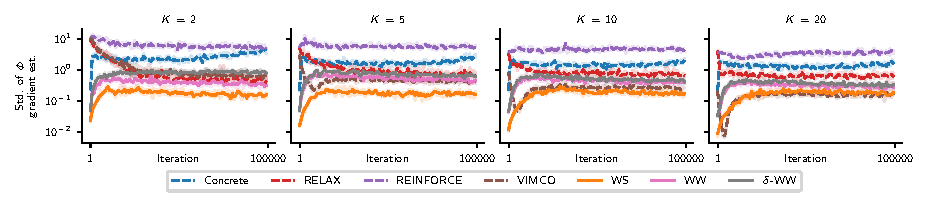
\includegraphics[width=\textwidth]{figures/gmm/errors_just_std.pdf}
  \vspace*{-4ex}
  \caption{
    Standard deviation of gradient estimator of $\phi$ for \gls{GMM}.
    Median and interquartile ranges from $10$ repeats shown.
    \Gls{WW} and \gls{WS} have lower-variance gradient estimators of $\phi$ than \gls{IWAE} except \gls{VIMCO}, as they avoid the high-variance term \circled{1} in \eqref{eq:iwae-reinforce}.
    This is a necessary, but not sufficient, condition for efficient learning, with other factors being gradient direction and the ability to escape local optima.
    The standard deviation of $\phi$'s gradient estimator is given by $\frac{1}{D_\phi} \sum_{d = 1}^{D_\phi} \std(g_d)$ where $g_d$ is the $d$th (out of $D_\phi$) element of one of $\phi$'s gradient estimators (e.g. \cref{eq:iwae-reinforce} for \acrshort{REINFORCE}) and $\std(\cdot)$ is estimated using $10$ samples.
  }
  \label{fig:gmm_just_std}
  \vspace*{-2ex}
\end{figure*}

\subsection{ADDITIONAL RESULTS}
\label{app:gmm/additional}

Here, we include additional \gls{GMM} experiments:
one for studying $\phi$'s gradient variance (\cref{fig:gmm_just_std}),
the other for comparing performances of the generative model and inference networks when $\theta$ is initialized closer to $\theta^*$ than in the main paper (\cref{fig:gmm_init_near}).

\Gls{WW} and \gls{WS} have lower variance gradient estimators than \gls{IWAE}, except \gls{VIMCO}.
%
This is because $\phi$'s gradient estimators for \gls{WW} and \gls{WS} do not include the high-variance term \circled{1} in \cref{eq:iwae-reinforce}.
%
This is a necessary but not sufficient condition for efficient learning with other important factors being gradient direction and the ability to escape local optima.
%
Employing the Concrete distribution gives low-variance gradients for $\phi$ to begin with, but the model learns poorly due to the high gradients bias (due to high temperature hyperparameter).

In \cref{fig:gmm_init_near}, we initialize $\theta$ so that the mixture probabilities are constant.
This means that the data bias is smaller than in the main paper's setting.
With smaller data bias, we expect \gls{WS} to perform better.
This is empirically verified since \gls{WS} outperforms other methods, including \gls{WW}.


\begin{figure*}[!ht]
  \centering
  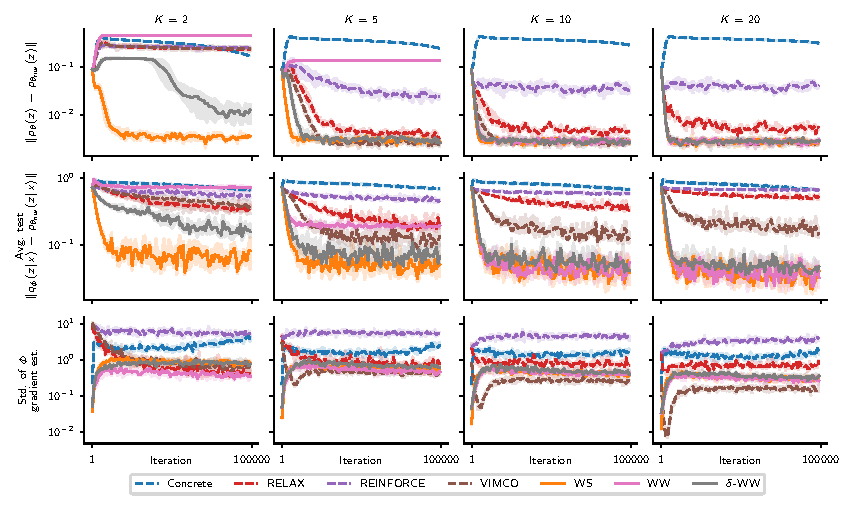
\includegraphics[width=\textwidth]{figures/gmm/errors_near.pdf}
  \vspace*{-4ex}
  \caption{
    \Gls{GMM} training when $p_\theta(x)$ is close to $p_{\theta^*}(x)$.
    \Gls{WS} outperforms other methods including \gls{WW} in generative model (top) and inference network (middle) learning.
    \Gls{VIMCO} has the lowest gradient variance (bottom) but still performs worse than \gls{WS} and results in worsening of the inference network as number of particles is increased.
  }
  \label{fig:gmm_init_near}
  \vspace*{-2ex}
\end{figure*}

\section{SIGMOID BELIEF NETWORKS}
\label{app:sigmoid_belief_nets}

In \cref{fig:sbn}, we show training of sigmoid belief networks with three stochastic layers with the same architecture as in \citet{mnih2016variational}.
We additionally drive number of particles up to $K = 5000$ and include \gls{KL} plots.
We find that in high particle regimes, model learning is virtually the same for \gls{WW} and \gls{VIMCO}.
However, \gls{WW} outperforms \gls{VIMCO} in terms of inference network learning.

\begin{figure*}[!ht]
  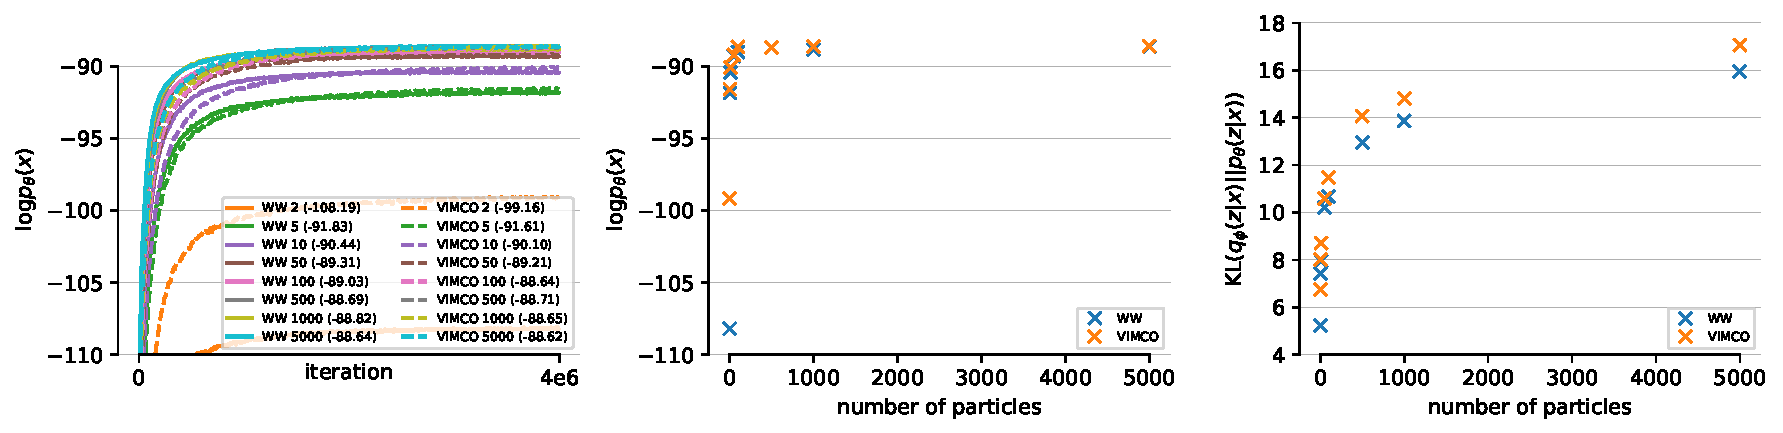
\includegraphics[width=\textwidth]{figures/discrete_vae/rws_baselines.pdf}
  \vspace*{-4ex}
  \caption{
    Training of sigmoid belief nets.
    \emph{(Left)}
    Training curves:
    \gls{WW} learns faster than \gls{VIMCO} but results in equal or slightly worse end test log likelihood.
    \emph{(Middle)}
    Log evidence values at the end of training:
    \gls{VIMCO} is slightly better than \gls{WW} in low-particle regimes but virtually the same in high-particle regimes.
    \emph{(Right)}
    \gls{KL} divergence at the end of training:
    \gls{WW} results in much lower \gls{KL} divergence than \gls{VIMCO}.
  }
  \label{fig:sbn}
  \vspace*{-2ex}
\end{figure*}

\section{DISCRETE VAES}
\label{app:dvae}

Rolfe 2016 \citep{rolfe2016dvae} introduces discrete \textsc{vae} (\textsc{dvae}).
It combines a prior over binary latent variables with an element-wise spike-and-X smoothing transformation, allowing approximate marginalization of the discrete variables.
This results in a continuous relaxation of discrete variables and a low-variance gradient estimator.
\citet{vahdat2018dvaepp} replaced the original transformation with an overlapping exponential transformation, leading to a yet lower-variance gradient estimator.
While both approaches produce relaxed binary variables, the relaxation is  significantly less tight (\cite{vahdat2018dvaepp}, Appendix C, Figure 5.) then the \textsc{concrete} of \cite{jang2017categorical,maddison2017concrete}
Both approaches require analytical inverse \textsc{cdf}s of the smoothing transformations, a shortcoming addressed by \citet{vahdat2018dvaehash} --- it also leads to a tighter relaxation than its predecessors, however no comparison to \textsc{concrete} is available.

\textsc{Dvae} was designed for undirected binary priors, \textit{e.g.}\ restricted Boltzmann machines (\textsc{rbm}), and it does not account for the case of categorical latent variables.
It is possible to construct a $d$-dimensional categorical variable from  $d-1$ binary variables via stick-breaking construction.
This process is slow, however, as it requires $\operatorname{\mathcal{O}}(d)$ sequential operations and cannot be parallelized.
Moreover, in the case of relaxed variables, the tightness of the derived relaxed categorical variable decreases exponentially with the number of dimensions.
This is a major issue in control flows: not only we have to evaluate all branches of the control flow, but the indicator variables that we multiply with outcomes of different branches become exponentially loose with the depth of the flow.


% \section{List of acronyms}
% \renewcommand{\glossarysection}[2][]{}
% \printglossary[type=\acronymtype]


\end{document}

%%% Local Variables:
%%% mode: latex
%%% TeX-master: t
%%% End:
